%latex提供的标题命令有如下九个。注意部分标题命令仅能在特定文类中使用。
    %\part
    %\chapter (report style only)
    %\section
    %\subsection
    %\subsubsection
    %\paragraph
    %\subparagraph
    %\subsubparagraph (milstd and book-form styles only)
    %\subsubsubparagraph (milstd and book-form styles only)
%空行代表重启一个段落。
\chapter{IFT46\ 基体和纤毛定位序列的鉴定}
%直接在奇数页页眉中显示章标题会多出一些章标题内部编号,这里重新定义\leftmark,后续所有章节都要重新定义
\renewcommand{\leftmark}{第四章\quad IFT46\ 基体和纤毛定位序列的鉴定}
\section{引言}
许多纤毛蛋白,尤其是纤毛膜蛋白,包含纤毛定位序列\
\citep{Hurd2011,Corbit2005,Berbari2008,Dishinger2010,McIntyre2015,Santos2014}。这些纤毛定位序列介导了纤毛蛋白的基体和纤毛定位。然而,纤毛定位序列本身存在多样性\
\citep{Malicki2014,Bhogaraju2013}。这表明多个不同的蛋白靶向系统参与了纤毛蛋白的基体和纤毛定位。已经鉴定的纤毛定位序列包括\ GPCRs\ 的第三个胞内环、Ax(S/A)xQ、RVxP、核定位信号以及\ SUMOylation\ 等\ \citep{Malicki2014,Bhogaraju2013,McIntyre2015,Dishinger2010,Berbari2008,Hurd2011,Santos2014,Corbit2005}。 然而在\ IFT\ 蛋白尤其是\ IFT46\ 中并未发现类似的定位序列。为此我们拟采用表达截短片段的方式来鉴定\ IFT46\ 的基体和纤毛定位序列。

\section{材料与方法}
\subsection{本研究所用仪器、试剂、培养基及溶液}
如未在正文中特别说明,本研究所用仪器、试剂、培养基及溶液信息均列于附录部分。其中,仪器信息列于
第\ \pageref{appen:A}\ 页的附录\ A,试剂信息列于第\ \pageref{appen:B}\ 页的附录\ B,培养基信息列于第\ \pageref{appen:C}\ 页的附录\ C,溶液信息列于第\ \pageref{appen:D}\ 页的附录\ D。

\subsection{藻细胞株及菌株的培养}
本章实验所用藻株有\ CC-125\index{CC-125}\ 和\ \textit{ift46-1}\index{\textit{ift46-1}}。通过电转化、筛选获得的藻株列于第\ \pageref{appen:E}\ 页的附录\ E。培养条件及方法参考第\
\pageref{subsec:algae}\ 页\ \ref{subsec:algae}\ 部分。大肠埃希氏菌
\index{大肠杆菌}\ DH5$\upalpha$\ 菌株由本实验室保存。培养条件及方法参考第\ \pageref{subsec:algae}\ 页
\ \ref{subsec:algae}\ 部分。

\subsection{计算机辅助分析}
使用\ PSIPRED\footnote{http://bioinf.cs.ucl.ac.uk/psipred/}\ \citep{Buchan2013,Jones1999,Bryson2005,Buchan2010,McGuffin2000}\ 预测\ IFT46\ 的二级结构和结构域边界。使用\ GeneSilico Metadisorder \citep{Kozlowski2012}\ 预测\ IFT46\ 的动态无序区。用\ COILS Server \citep{Lupas1991}\ 预测\ IFT46\ 形成卷曲螺旋的概率。蛋白质理论分子量通过\ ExPASy\footnote{Expert Protein Analysis System}\ 中的\ Compute pI/Mw\footnote{http://web.expasy.org/compute\_pi/}\ 进行预测,其中“分辨率”选项设置为“平均”。

\textit{IFT46}\ 的基因组\ DNA\ 及蛋白序列均来源于\ Joint Genome Institute Phytozome 12\footnote{https://phytozome.jgi.doe.gov/pz/portal.html}\ 中的\
\textit{Chlamydomonas reinhardtii} v5.5\ 数据库。团藻\ (XP\_002950030)、智人\ (NP\_001\allowbreak 162089)、 小鼠\ (NP\_076320)、 秀丽隐杆线虫\ (NP\_001076770)、爪蟾\ (NP\_001090393)、 黄牛\ (NP\_001068677)、家犬\ (XP\_536553)、大鼠\ (NP\_001019931)、鸡\ (XP\_417918)、 斑马鱼\ (XP\_003199413)、 紫海胆\ (XP\_795443)、日本血吸虫\ (Q5DHJ5)、球石藻(颗石藻)\ (XP\_005763582)、 嗜热四膜虫\ (XP\_001017111)以及蜜蜂\ (XP\_006565024)\ 的\ IFT46\ 蛋白序列均来源于\ NCBI\footnote{National Center for Biotechnology Information}。用\ Clustal W \citep{Larkin2007}\ 对\ IFT46\ 进行多重序列比对,比对后的序列在\ CLC Sequence Viewer 7.7\footnote{CLC bio, QIAGEN}\ 中进行着色。

\subsection{分子克隆}\label{subsec:melcular cloning second}
如未作特殊说明,分子克隆所用方法参考第\ \pageref{subsec:melcular cloning}\ 页\
\ref{subsec:melcular cloning}\ 部分。

\subsubsection{重叠延伸\ PCR}\label{subsec:SOEPCR}
%开始图片浮动体环境,其中!表示取消严谨限制,h表示在此处插入,t表示在本页或下一页顶部插入
\begin{figure}[!ht]
%居中对齐
\centering
%设置图片搜索路径,每个路径用{}括起来
\graphicspath{{figures/}}
%插入图片并设置图片宽度为文本宽度减10mm
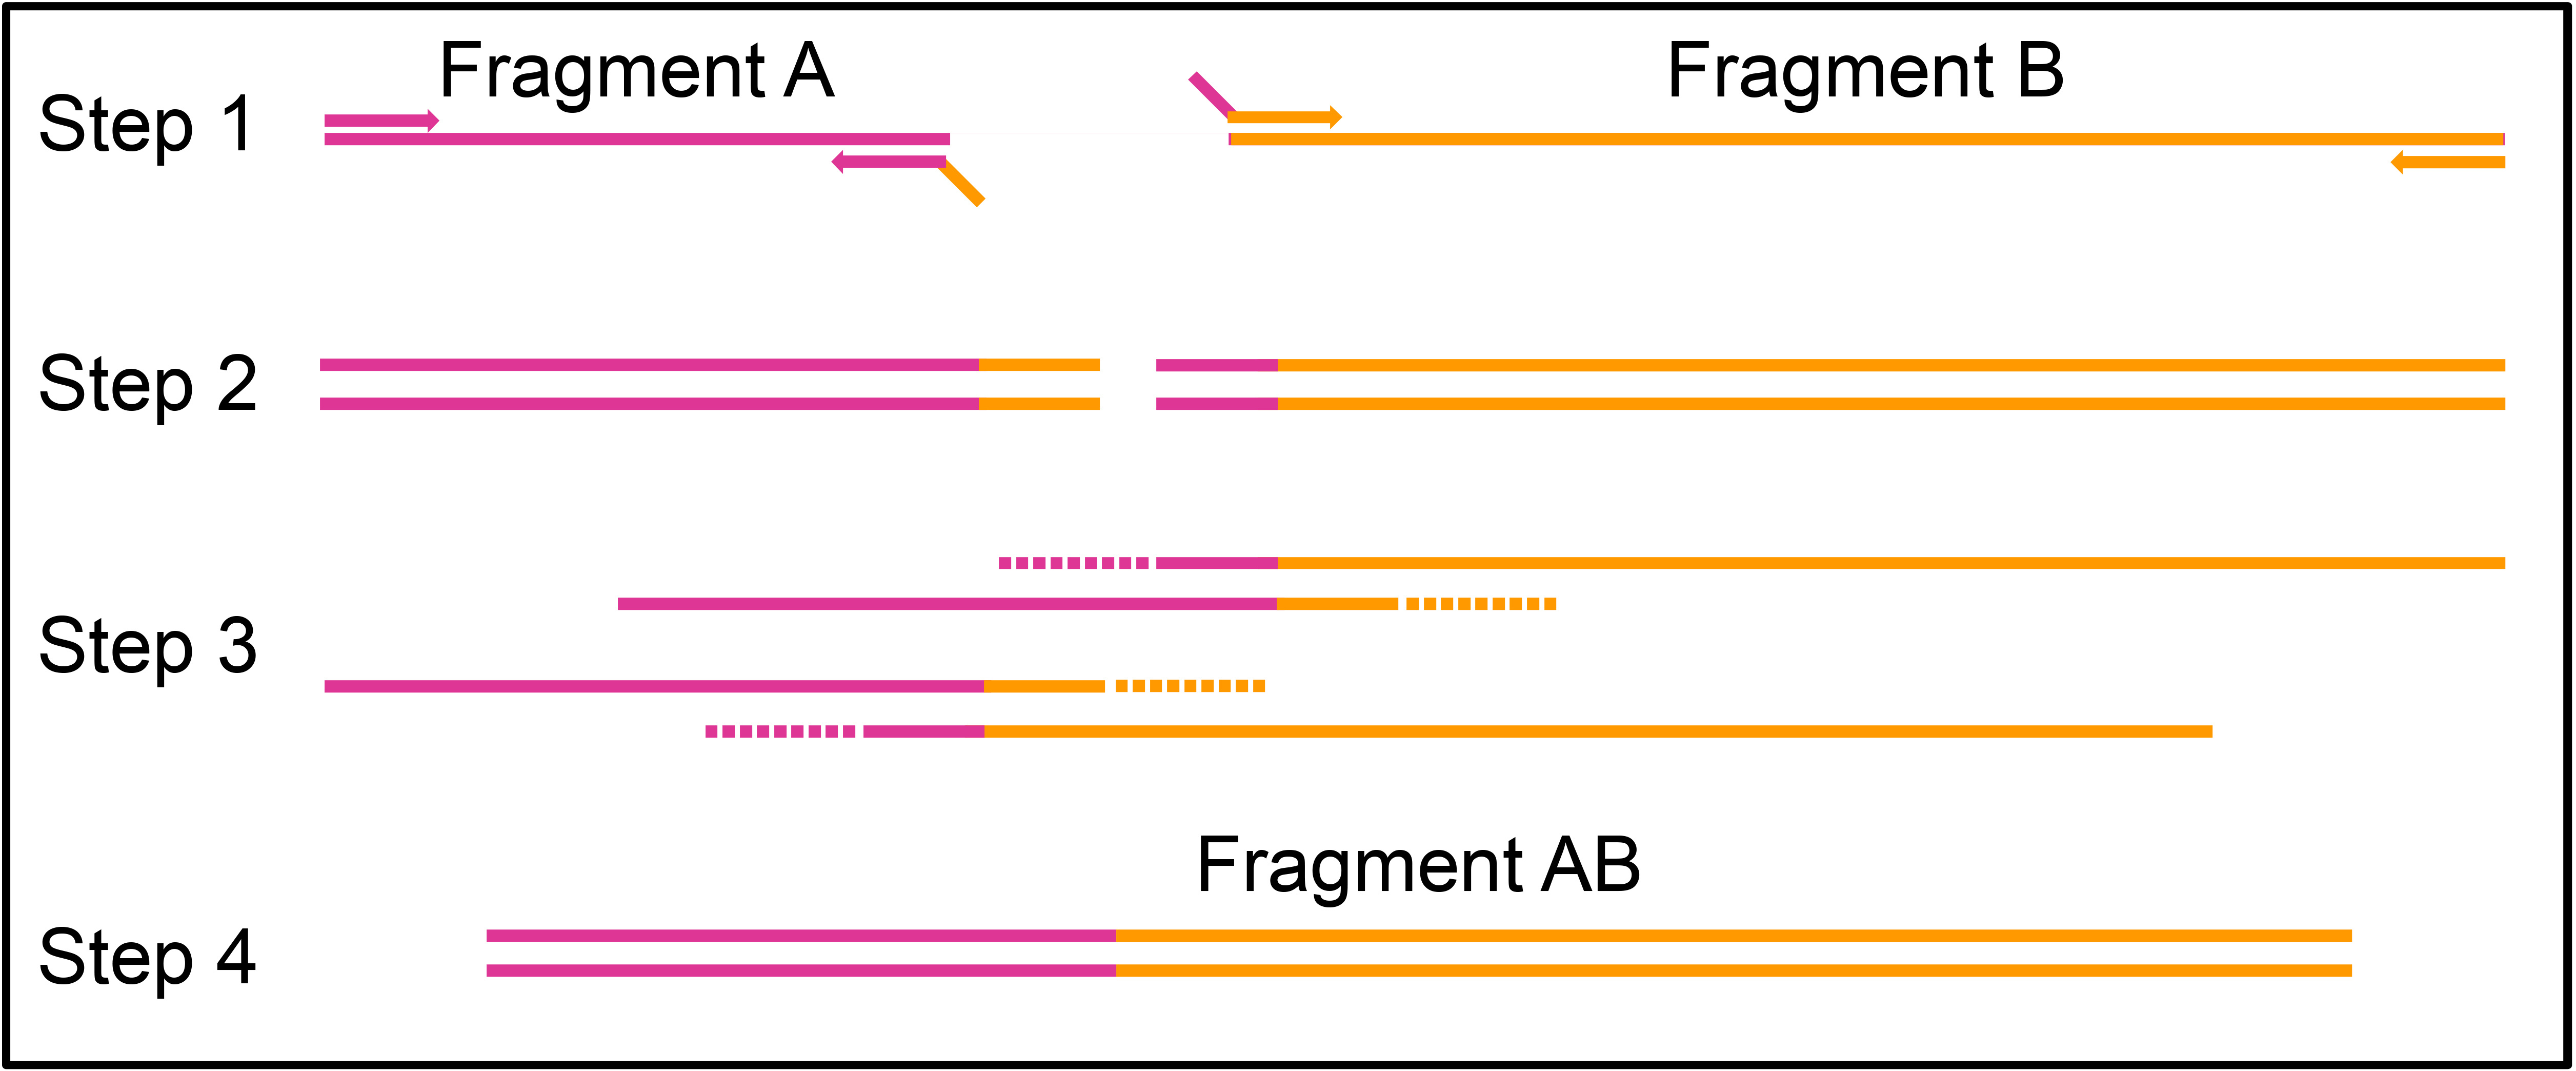
\includegraphics[width=\textwidth]{fig4-1.jpg}
%生成中英双语标题
{\setstretch{1.667}
\bicaption[fig:4.1]{图}{重叠延伸\ PCR\ 的基本原理。第一步,独立扩增片段\ A\ 和片段\ B;第二步,电泳回收获得纯化的片段\ A\ 和片段\ B;第三步,片段\ A\ 和片段\ B\ 互为引物和模板进行重叠延伸扩增;第四步,电泳回收获得纯化的片段\ AB。}{Figure}{Principle of splicing by overlap extension PCR. Step 1, amplify fragment A and B; Step 2, purify fragment A and B; Step 3, overlap extension PCR of fragment A and B; Step 4, purify fragment AB.}
\par}
%结束图片浮动体环境
\end{figure}
为了使用\ \textit{IFT46}\ 自身的启动子表达\ IFT46\ 的\ C\ 端,我们需要使用重叠延伸\ PCR\ \citep{Quan2011,Quan2009,Bryksin2010}。其基本原理如图\ \ref{fig:4.1}\ 所示:首先分别扩增片段\ A\ 和片段\ B,将回收得到的两个片段按\ 1:1\ 的摩尔比作为引物和模板加入到\ PCR\ 体系中进行二次扩增。为了保证获得足够质量的片段\ AB,这里至少需要加入\ \SI{200}{\ng}\ 的短片段\ A。由于片段\ A\ 和片段\ B\ 含有重叠部分,二者在扩增过程中互为引物和模板。对扩增产物进行电泳并回收目的条带即可用于\ TA\ 克隆。若片段\ AB\ 两端带有酶切位点,可先用限制性内切酶进行切割。酶切产物经纯化后可用于连接反应。

\subsubsection{利用寡核苷酸退火合成双链\ DNA}\label{subsec:oligoanneal}
为了快速经济的合成较短的双链\ DNA,我们可以通过将寡核苷酸退火来实现\ \citep{Hu2014}。其基本原理如图\ \ref{fig:4.2}\ 所示:将目标\ DNA\ 截断为八个片段,片段之间存在至少\ 15 bp\ 的重叠区域。分别合成八个寡核苷酸片段并用去离子水溶解至终浓度为\ \SI{100}{\milli\nauticalmile}。按表\ \ref{tab:table4.1}\ 加入试剂并利用\ PCR\ 仪按表\ \ref{tab:table4.2}\ 进行反应。取反应产物进行电泳并回收目的条带即为所需要的双链\ DNA。 在实际操作过程中,寡核苷酸的条数不一定为八,只要保证单条引物的长度不操过\ 59 bp\ 且存在\ 15 bp\ 以上的重叠区域即可。此外,利用这种方法合成的双链\ DNA\ 可以含平末端或粘性末端。这意味着合成产物不需要经过酶切步骤即可用于连接反应。
%开始图片浮动体环境,其中!表示取消严谨限制,h表示在此处插入,t表示在本页或下一页顶部插入
\begin{figure}[t]
%居中对齐
\centering
%设置图片搜索路径,每个路径用{}括起来
\graphicspath{{figures/}}
%插入图片并设置图片宽度为文本宽度减10mm
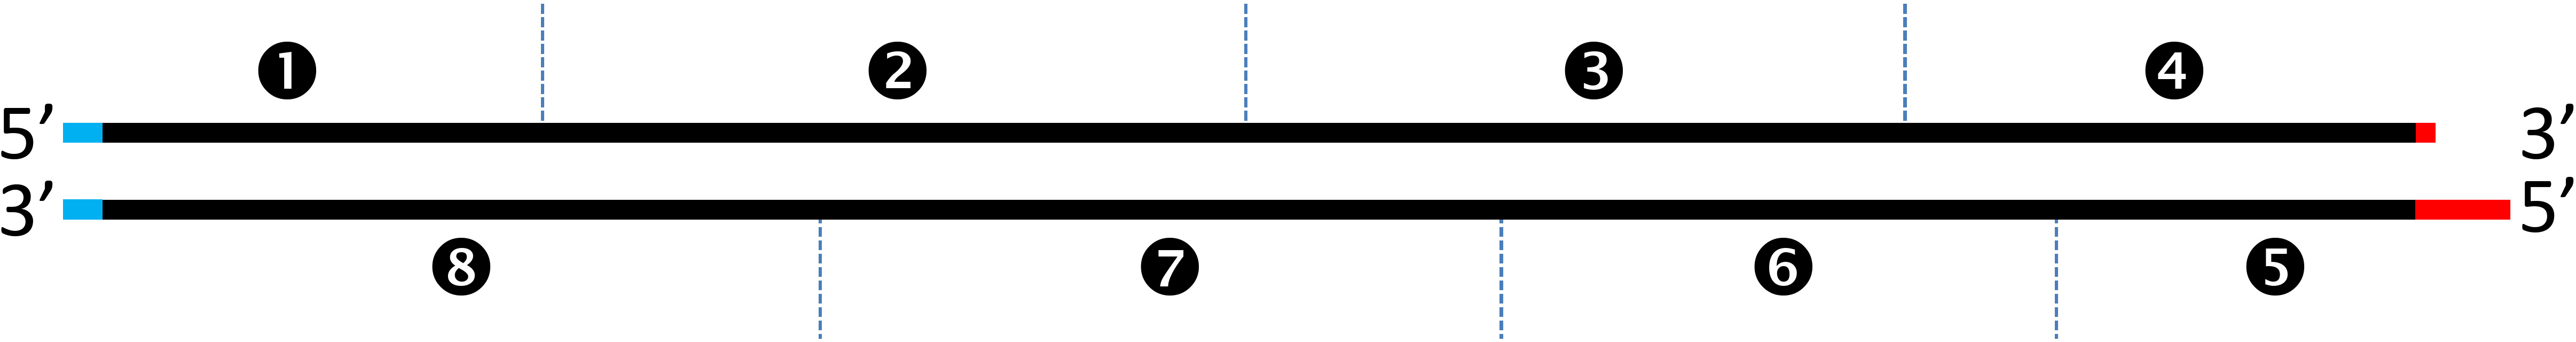
\includegraphics[width=\textwidth]{fig4-2.jpg}
%生成中英双语标题
{\setstretch{1.667}
\bicaption[fig:4.2]{图}{利用寡核苷酸退火合成双链\ DNA\ 的原理示意图。数字代表不同的寡核苷酸,蓝色虚线代表截断位点。}{Figure}{Principle of rapid construction of double strand DNA using oligonucleotides. Numbers indicate different oligonucleotides. Blue dashed lines mark the truncated sites.}
\par}
%结束图片浮动体环境
\end{figure}

%开始表格浮动体环境,其中!表示取消严谨限制,h表示在此处插入,t表示在本页或下一页顶部插入s
\begin{table}[!ht]
%居中对齐
\centering
%生成中英双语标题
{\setstretch{1.667}
\bicaption[tab:table4.1]{表}{利用寡核苷酸退火合成双链\ DNA\ 反应体系}{Table}{System of rapid construction of double strand DNA using oligonucleotides}
\par}
%更改表格内文字的字号
\small
%开始绘制表格
\begin{tabular*}{\textwidth}[c]{@{\extracolsep{\fill}}lll}
%绘制一条水平线
\toprule
编号\ (Number) & 试剂\ (Reagents) & 体积\ (Volume)\\
\midrule
1 & 10xAnnealing buffer for DNA oligos & 5 $\upmu$L\\
2 & \SI{100}{\milli\nauticalmile} Oligo 1 & 5 $\upmu$L\\
3 & \SI{100}{\milli\nauticalmile} Oligo 2 & 5 $\upmu$L\\
4 & \SI{100}{\milli\nauticalmile} Oligo 3 & 5 $\upmu$L\\
5 & \SI{100}{\milli\nauticalmile} Oligo 4 & 5 $\upmu$L\\
6 & \SI{100}{\milli\nauticalmile} Oligo 5 & 5 $\upmu$L\\
7 & \SI{100}{\milli\nauticalmile} Oligo 6 & 5 $\upmu$L\\
8 & \SI{100}{\milli\nauticalmile} Oligo 7 & 5 $\upmu$L\\
9 & \SI{100}{\milli\nauticalmile} Oligo 8 & 5 $\upmu$L\\
10& ddH$_2$O  & To 50 $\upmu$L\\
\bottomrule
%结束绘制表格
\end{tabular*}
%结束表格浮动体环境
\end{table}

%开始表格浮动体环境,其中!表示取消严谨限制,h表示在此处插入,t表示在本页或下一页顶部插入
\begin{table}[!ht]
%居中对齐
\centering
%生成中英双语标题
{\setstretch{1.667}
\bicaption[tab:table4.2]{表}{利用寡核苷酸退火合成双链\ DNA\ 反应程序}{Table}{Program of rapid construction of double strand DNA using oligonucleotides}
\par}
%更改表格内文字的字号
\small
%开始绘制表格
\begin{tabular*}{\textwidth}[c]{@{\extracolsep{\fill}}lll}
%绘制一条水平线
\toprule
步骤\ (Steps) & 温度\ (Temperature) & 反应时间\ (Reaction Time)\\
\midrule
1 & \SI{94}{\degreeCelsius} & 5 \minute\\
2 & \SI{80}{\degreeCelsius} & 10 \minute\\
3 & \SI{75}{\degreeCelsius} & 10 \minute\\
4 & \SI{70}{\degreeCelsius} & 10 \minute\\
5 & \SI{65}{\degreeCelsius} & 10 \minute\\
6 & \SI{60}{\degreeCelsius} & 10 \minute\\
7 & \SI{55}{\degreeCelsius} & 10 \minute\\
8 & \SI{50}{\degreeCelsius} & 10 \minute\\
9 & \SI{40}{\degreeCelsius} & 5 \minute\\
10 & \SI{30}{\degreeCelsius} & 5 \minute\\
11 & \SI{20}{\degreeCelsius} & 5 \minute\\
12 & \SI{10}{\degreeCelsius} & $\infty$\\
\bottomrule
%结束绘制表格
\end{tabular*}
%结束表格浮动体环境
\end{table}

\subsubsection{质粒抽提}
使用\ GeneMark\ 质粒小量纯化试剂盒进行质粒提取,具体步骤如下。

(1)取\ 5-10 mL\ 过夜培养的菌液,16800 g\ 室温离心一分钟,尽量吸除上清。

(2)向留有菌体沉淀的离心管中加入\ \SI{200}{\uL}\ Solution I,使用移液器悬浮细菌沉淀。

(3)向离心管中加入\ \SI{200}{\uL}\ Solution II\ 温和的上下翻转五次使菌体充分裂解。

(4)向离心管中加入\ \SI{200}{\uL}\ Solution III\ 温和的上下翻转五次混合均匀。

(5)16800 g\ 室温离心五分钟。此时离心管底部有白色沉淀。

(6)将\ spin column\ 装入\ collection tube\ 中,用移液器将上清转移到\ spin column\ 中,12000 g\ 室温离心一分钟,倒掉\ collection tube\ 中的废液后将\ spin column\ 放回\ collection tube\ 中。

(7)向\ spin column\ 中加入\ \SI{700}{\uL}\ Wash solution,12000 g\ 室温离心一分钟,倒掉\ collection tube\ 中的废液后将\ spin column\ 放回\ collection tube\ 中。重复该过程一次。

(8)将\ spin column\ 放入\ collection tube\ 中,16800 g\ 室温离心三至五分钟以除去残余的酒精。

(9)将\ spin column\ 置于干净的离心管中,向吸附膜中央滴加\ \SI{50}{\uL}\ Elution solution,室温放置两分钟后\ 12000 g\ 室温离心一分钟将质粒溶液收集到离心管中。

(10)使用微量紫外分光光度计(Quawell-Q5000)测定\ DNA\ 的浓度和纯度。\SI{-20}{\degreeCelsius}保存质粒溶液。

\subsubsection{大肠杆菌感受态细胞的快速制备}
大肠杆菌感受态细胞的快速制备方法如下。

(1)配置\ SOB\ 培养基并用\ \SI{1}{\L}\ 的三角瓶分装为\ \SI{250}{\mL}\ 每瓶,高温高压灭菌后备用。取出\ \SI{-80}{\degreeCelsius}\ 保存的\ TOP10、DH5$\upalpha$、DH10$\upbeta$\ 或其他菌种用接种环蘸取少量菌液,在无抗性的\ LB\ 固体培养基平板上划线,将平板倒置于\ \SI{37}{\degreeCelsius}\ 培养箱中培养过夜。

(2)挑取一个单菌落接种至\ \SI{5}{\mL}\ 无抗性的\ LB\ 液体培养基中,\SI{37}{\degreeCelsius}\ 震荡培养过夜。

(3)向每瓶\ SOB\ 培养基中加入\ 2 M\ 的\ MgCl$_2$\ 溶液\ \SI{1.25}{\mL}。取\ \SI{2}{\mL}\ 新鲜的菌液转接到\ \SI{250}{\mL}\ 无抗性的\ SOB\ 液体培养基中,\SI{37}{\degreeCelsius}\ 震荡培养至\ OD600\ 为\ 0.3-0.4。

(4)取出菌液于冰上静置十分钟。此过程中将\ MgCl$_2$$\cdot$CaCl$_2$\ 溶液置于冰上预冷。使用\ \SI{50}{\mL}\ 离心管\ 2700 g \SI{4}{\degreeCelsius}\ 离心十分钟,弃上清。

(5)细胞沉淀用\ \SI{100}{\mL}\ 预冷的\ MgCl$_2$$\cdot$CaCl$_2$\ 溶液重悬,以同样的参数再次离心十分钟,弃上清。

(6)细胞沉淀用\ \SI{10}{\mL}\ 预冷的\ CaCl$_2$$\cdot$甘油溶液重悬。轻轻混匀后分装至\ \SI{1.5}{\mL}\ 离心管中,每管\ \SI{200}{\uL}。立即将分装好的感受态细胞冻存在液氮中,分装完毕后迅速转移到\ \SI{-80}{\degreeCelsius}\ 冰箱中。

\subsubsection{构建表达\ IFT46\ 截短片段的载体}
为了表达\ IFT46\ 的截短片段,我们构建了\ pHK231,pHK232,pHK233,pHK243,pHK244\ 和\ pHK245。 这些载体在衣藻中分别表达\ IFT46-N1,IFT46-N,IFT46$\Delta$C1,IFT46$\Delta$N1,IFT46-C\ 和\ IFT46-C1。 以\ pGEM-T Easy-\textit{IFT46}\ 为模板,用引物\ ACE-F\ 和\ A-R\ 扩增获得\
\textit{IFT46-N1}\ 的编码序列,扩增产物使用\ \textit{Nde}I\ 和\ \textit{Eco}RV\ 酶切后插入到\
\textit{Nde}I/\textit{Eco}RV\ 消化后的\ pHK86\ 中获得\ pHK231。表达\ IFT46-N(pHK232)和\ IFT46$\Delta$C1 (pHK233)的载体使用类似的方法进行构建,但使用的引物对分别为\ ACE-F/C-R\ 和ACE-F/E-R。为了获得能够表达\ IFT46$\Delta$N1\ 的序列,我们需要\ \textit{IFT46}\ 的启动子和\ IFT46$\Delta$N1\ 的编码区两个元件。以\ pGEM-T Easy-\textit{IFT46}\ 为模板,使用引物\ ACE-F\ 和\ B-R\ 进行扩增可获得\ \textit{IFT46}\ 的启动子序列,使用引物\ B-F\ 和\ IFT46-R\ 进行扩增可获得\ IFT46$\Delta$N1\ 的编码区序列。利用重叠延伸\ PCR(参考第\ \pageref{subsec:SOEPCR}\ 页\
\ref{subsec:SOEPCR}\ 部分)将两个元件融合后用\ \textit{Nde}I\ 和\ \textit{Eco}RV\ 双酶切并连接到\ \textit{Nde}I/\textit{Eco}RV\ 消化后的\ pHK86\ 中,由此获得表达\ IFT46$\Delta$N1\ 的\ pHK243。 除引物不同外,pHK244\ 和\ pHK245\ 的构建过程与\ pHK243\ 类似。在\ pHK244\ 的构建过程中,使用引物对\ ACE-F/D-R\ 扩增\ \textit{IFT46}\ 的启动子区,使用引物对\ D-F/IFT46-R\ 扩增IFT46-C\ 的编码区。在\ pHK245\ 的构建过程中,使用引物对\ ACE-F/F-R\ 扩增\ \textit{IFT46}\ 的启动子区,使用引物对\ F-F/IFT46-R\ 扩增\ IFT46-C1\ 的编码区。

为了表达\ IFT46-C1\ 的截短片段,我们构建了\ pHK308,pHK310,pHK309,pHK311,pHK312\ 和\ pHK313。 这些载体在衣藻中分别表达\ BBTS1,BBTS2,BBTS3,BBTS4,BBTS5\ 和\ BBTS6。以\ pHK245\ 为模板,用引物\ BBTS-F/BBTS1-R\ 扩增获得\ \textit{BBTS1}\ 的编码序列,扩增产物经\
\textit{Nde}I/\textit{Eco}RV\ 酶切后克隆至\ \textit{Nde}I/\textit{Eco}RV\ 消化的\ pHK245,由此获得表达\ BBTS1\ 的\ pHK308。pHK310\ 的构建过程与\ pHK308\ 的构建方法类似,不同之处在于使用了引物\ BBTS-F\ 和\ BBTS3-R。 为了构建\ pHK309,我们需要\ \textit{IFT46}\ 的启动子和\ \textit{BBTS2}\ 的编码区两个元件。以\ pHK245\ 为模板,使用引物\ BBTS-F\ 和\ BBTS2-R\ 进行扩增可获得\ \textit{IFT46}\ 的启动子序列,使用引物\ BBTS2-F\ 和\ IFT46-R\ 进行扩增可获得\ \textit{BBTS2}\ 的编码区序列。利用重叠延伸\ PCR (参考
第\ \pageref{subsec:SOEPCR}\ 页\ \ref{subsec:SOEPCR}\ 部分)将两个元件融合后用\ \textit{Nde}I 和
\textit{Eco}RV\ 双酶切并连接到\ \textit{Nde}I/\textit{Eco}RV\ 消化后的\ pHK245\ 中,由此获得表达\ BBTS2\ 的\ pHK309。pHK311、pHK312\ 和\ pHK313\ 的构建过程与\ pHK309\ 类似。在\ pHK311\ 的构建过程中,使用引物对\ BBTS-F/BBTS4-R\ 扩增\ \textit{IFT46}\ 的启动子区,使用寡核苷酸\ BBTS4-1、BBTS4-2、BBTS4-3、BBTS4-4\ 和\ BBTS4-5\ 退火合成\ \textit{BBTS4}\ 的编码区(参考
第\ \pageref{subsec:oligoanneal}\ 页\ \ref{subsec:oligoanneal}\ 部分)。在\ pHK312\ 的构建过程中,使用引物对\ BBTS-F/BBTS5-R1\ 扩增\ \textit{IFT46}\ 的启动子区,使用引物对\ BBTS5-F/BBTS5-R2\ 扩增\ \textit{BBTS5}\ 的编码区。在\ pHK313\ 的构建过程中,使用引物对\ BBTS-F/BBTS6-R\ 扩增
\textit{IFT46}\ 的启动子区,使用寡核苷酸\ BBTS6-6、BBTS6-7、BBTS4-2、BBTS4-3\ 和\ BBTS4-5\ 退火合成\ \textit{BBTS6}\ 的编码区。

克隆所用载体以及构建的载体的详细信息见第\ \pageref{appen:F}\ 页的附录\ F,克隆所用引物信息见
第\ \pageref{appen:G}\ 页的附录\ G。

\subsection{衣藻电转化}
参考第\ \pageref{subsec:electrotransformation}\ 页\ \ref{subsec:electrotransformation}\ 部分。

\subsection{鞭毛提取}\label{subsec:flagella}
参考\ \citet{Behal2013}、\citet{Cole1998}、\citet{Richey2013}\ 和\ \citet{Witman1972}\ 等人的方法并稍作修改,具体步骤如下。

(1)培养\ \SI{100}{\mL}\ 藻细胞至对数生长期。

(2)将\ \SI{200}{\mL}\ 藻液转接到\ \SI{5}{\L}\ 液体\ TAP\ 培养基中,曝气培养至细胞浓度达
\num{5.0d7}\ cells/mL。\SI{3500}{\g}\ 室温离心五分钟,弃上清,沉淀用\ \SI{1}{\L}\ \SI{10}{\milli\nauticalmile}\ HEPES\ 重悬。

(3)将细胞悬液转入\ \SI{1}{\L}\ 烧杯中,300 rpm搅拌光照培养两小时使其鞭毛恢复。\SI{3500}{\g}\ 室温离心五分钟,弃上清,沉淀用\ \SI{75}{\mL}\ \SI{10}{\milli\nauticalmile}\ HEPES\ 重悬。

(4)pH shock\ \citep{Lefebvre1995,Hunter2016}:用\SI{0.5}{\nauticalmile}\ HAc\ 调节\ pH\ 值至\ 4.5,等待三十秒待鞭毛脱落。立即用\ 0.5 M KOH\ 调节\ pH\ 值至\ 7.2,在显微镜下观察鞭毛是否脱落。

(5)将悬液置于冰上,加入\ \SI{30}{\mL}\ 含\ 25\%\ 蔗糖的\ \SI{10}{\milli\nauticalmile}\ HEPES\ 混匀。

(6)将细胞悬液转移到\ \SI{500}{\mL}\ 离心瓶中,用带长针管的注射器向其底部缓慢注入\ \SI{50}{\mL}\ 含\ 25\%\ 蔗糖的\ \SI{10}{\milli\nauticalmile}\ HEPES\ ,\SI{4}{\degreeCelsius}\ \SI{2500}{\g}\ 离心十分钟。将上清转移至\ \SI{50}{\mL}\ 离心管中,用注射器向离心管底部缓慢注入\ \SI{5}{\mL}\ 含\ 25\%\ 蔗糖的\ \SI{10}{\milli\nauticalmile}\ HEPES\ ,\SI{4}{\degreeCelsius}\ \SI{2500}{\g}\ 离心十分钟。

(7)将上清转移至\ \SI{50}{\mL}\ 圆底离心管中,\SI{4}{\degreeCelsius}\ \SI{10000}{\g}\ 离心十分钟,在管底可见乳白色沉淀即为提取出来的鞭毛,用\SI{100}{\uL}\ 含蛋白酶抑制剂(Sigma-Aldrich, \#P9599, U.S.)的\ 1xHMDEK\ 溶解后\ \SI{-80}{\degreeCelsius}\ 保存。

(8)如需要分离轴丝或纤毛膜、基质蛋白,使用含\ 0.1\%\ NP-40\ 和蛋白酶抑制剂的\ 1xHMDEK\ 溶解鞭毛沉淀,
\SI{4}{\degreeCelsius}\ 反应三十分钟后\ \SI{4}{\degreeCelsius}\ \SI{16800}{\g}\ 离心十分钟,沉淀即为轴丝蛋白,上清即为纤毛膜、基质蛋白。

\subsection{SDS-PAGE\ 及免疫印迹分析}
SDS-PAGE\ 参考第\ \pageref{subsec:SDS-PAGE}\ 页\ \ref{subsec:SDS-PAGE}\ 部分。免疫印迹分析参考
第\ \pageref{subsec:western}\ 页\ \ref{subsec:western}\ 部分。检测所用抗体的信息见第\
\pageref{appen:H}\ 页的附录\ H。

\subsection{显微观察}
显微观察及活细胞成像参考第\ \pageref{subsec:microscope}\ 页\ \ref{subsec:microscope}\ 部分。

\subsection{免疫共沉淀}\label{subsec:CoIP}
参考\ \citet{Richey2013}、\citet{Fowkes1998}\ 和\ \citet{Silva2012}\ 的方法并稍作修改,具体步骤如下。

(1)培养\ \SI{10}{\L}\ 藻细胞,参考第\ \pageref{subsec:flagella}\ 页\ \ref{subsec:flagella}\ 部分提取鞭毛。

(2)使用\ 500 $\upmu$L\ 含有蛋白酶抑制剂的\ 1xHMDEK\ 重悬鞭毛沉淀,利用
液氮和\ \SI{30}{\degreeCelsius}\ 温水冻融三次释放可溶性蛋白。

(3)\SI{4}{\degreeCelsius},16800 g\ 离心十分钟,收集上清。

(4)\SI{4}{\degreeCelsius}, 100000 g\ 离心十分钟进一步除去不可溶蛋白。重复该过程一次。

(5)用\ 1xHMDEK\ 缓冲液洗涤蛋白\ A\ 标记的琼脂糖珠\footnote{protein A-sepharose from Staphylococcus aureus, Sigma P3391}三次,用含\ 3\%\ BSA\ 的\ 1xHMDEK\ 缓冲液室温封闭琼脂糖珠一小时。

(6)取前面获得的纤毛膜/基质可溶性蛋白溶液\ 50 $\upmu$L,加入\ 30 $\upmu$L\ 抗\ HA\ 抗体,混匀后冰上孵育两小时。对照组加等体积的鼠\ IgG。

(7)取\ 20 $\upmu$L\ 处理过的琼脂糖珠加入到混合液中,\SI{4}{\degreeCelsius}旋转反应过夜。

(8)\SI{4}{\degreeCelsius},4000 g\ 离心一分钟收集琼脂糖珠,用\ 500 $\upmu$L\ 含\ 0.05\%\ NP-40\ 的\ 1xHMDEK\ 室温洗涤琼脂糖珠三次,每次三分钟。

(9)\SI{4}{\degreeCelsius},4000 g\ 离心一分钟收集琼脂糖珠,加入\ 25 $\upmu$L\ 的\ 2xLaemmli\ 上样缓冲液,沸水煮十分钟后立即置于冰上冷却。

(10)\SI{4}{\degreeCelsius},4000 g\ 离心一分钟收集上清即可用于免疫印迹检测。

\subsection{蔗糖密度梯度离心}
参考\ \citet{Fuhrmann1999}、\citet{Richey2012}、\citet{Behal2013}\ 和\ \citet{Richey2013}\ 的方法并稍做修改,具体步骤如下。

(1)培养\ 20 L\ 藻并提取鞭毛,鞭毛的提取方法参考第\ \pageref{subsec:flagella}\
页\ \ref{subsec:flagella}\ 部分。向提取的鞭毛中加\ 200 $\upmu$L\ 含有\ 0.5\%\ NP-40\ 和蛋白酶抑制剂的\ 1xHEMDEK\ 使之溶解。液氮冻融两次。

(2)涡旋反应十分钟后\ \SI{4}{\degreeCelsius},16800 g\ 离心十分钟。

(3)取上清\ 200 $\upmu$L\ 再次离心,取上清\ 150 $\upmu$L\ 再次离心得到\ 100 $\upmu$L\ 上清。此步勿多取,否则样品中所含不可溶蛋白将影响密度梯度离心且离心后管底含有大量不贴壁沉淀影响分装。余下的上清可以用作免疫印迹分析时的阳性对照。

(4)在\ MLS50\ 专用离心管中制备\ 25\%-20\%-15\%-10\%\ 蔗糖梯度,每个梯度各\ 500 $\upmu$L。制备方法为先铺高浓度蔗糖溶液,再依次铺低浓度蔗糖溶液。将离心管置于管套中盖上盖子,
\SI{4}{\degreeCelsius}\ 静置过夜待其通过自由扩散产生连续梯度。

(5)在蔗糖上方沿管壁缓慢加入\ 100 $\upmu$L\ 样品后用石蜡油补平至管口。为避免杂质对离心产生干扰,所用石蜡油需先经\ \SI{0.22}{\um}\ 滤膜过滤。

(6)\SI{4}{\degreeCelsius}, 200000 g\ 离心\ 4.5\ 个小时,取出离心管吸走石蜡油和样品层(样品层一般呈浅黄色)。用移液器每\ 80 $\upmu$L\ 沿管壁取样,总计分装二十四管。

(7)每管取\ 15 $\upmu$L\ 样品加\ 5 $\upmu$L\ 5xLoading buffer\ 在沸水中煮五分钟后立即置于冰上冷却三分钟。样品可立即用于\ SDS-PAGE\ 和免疫印迹分析,也可置于\ \SI{-20}{\degreeCelsius}\ 保存备用。

%开始图片浮动体环境,其中!表示取消严谨限制,h表示在此处插入,t表示在本页或下一页顶部插入
\begin{figure}[h!tbp]
%居中对齐
\centering
%设置图片搜索路径,每个路径用{}括起来
\graphicspath{{figures/}}
%插入图片并设置图片宽度为文本宽度减10mm
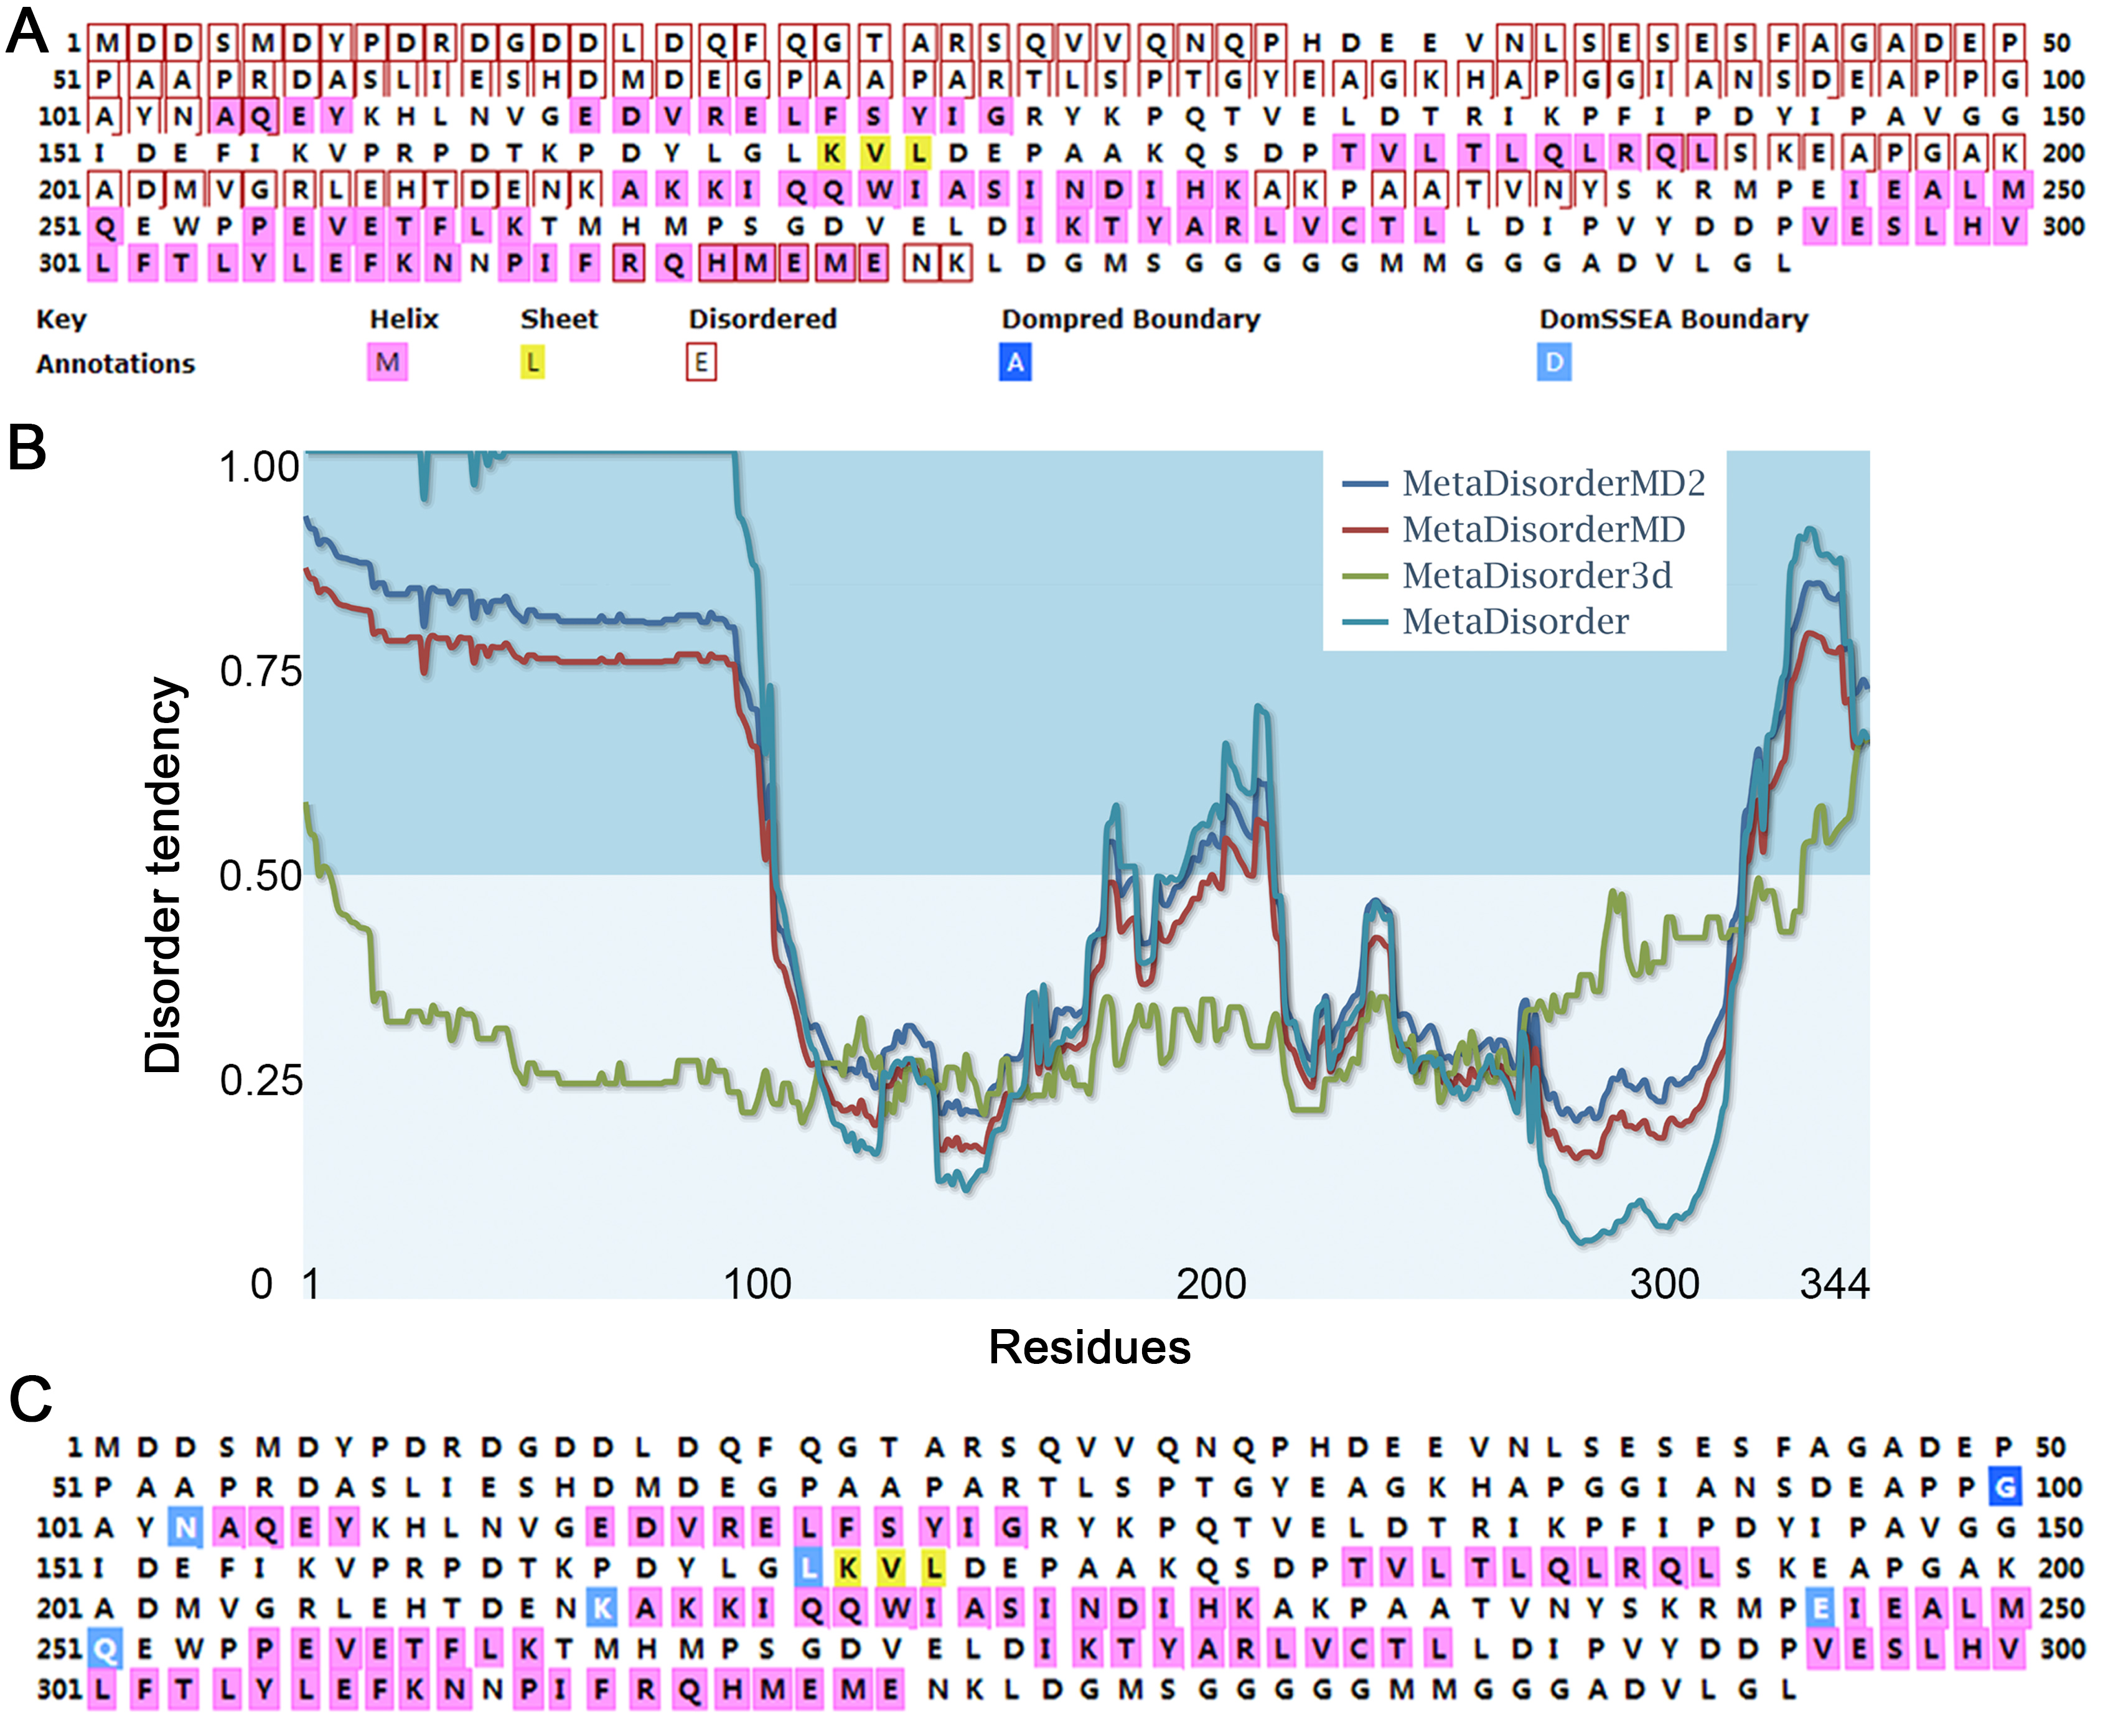
\includegraphics[width=\textwidth]{fig4-3.jpg}
%生成中英双语标题
{\setstretch{1.667}
\bicaption[fig:4.3]{图}{IFT46\ 二级结构和超二级结构预测。(A)IFT46\ 二级结构预测。各符号的含义列于图片下方。(B)蛋白无序趋势预测显示\ IFT46\ 的\ N\ 端和\ C\ 端为动态无序区。不同颜色的曲线为不同算法预测的结果,算法名称如图右上角所示。0.5\ 为动态无序的截断值。大于\ 0.5\ 的区域代表动态无序区,小于\ 0.5\ 的区域代表有序区。(C)使用\ PSIPRED DomPred\ 预测\ IFT46\ 可能的结构域边界。图中深蓝色和浅蓝色方块标注的位点即为可能的结构域边界。}{Figure}{Advanced structure predictions of IFT46. (A) Secondary structure prediction of IFT46. Meanings of symbols were given below. (B) Protein disorder prediction indicates that the N-terminus and the C-terminus tail of IFT46 are largely disordered. The curves with different colors show the prediction results of different algorithms whose names are given in the upper right corner of this panel. The line at 0.5 (vertical axis) is the cutoff for disorder ($>$ 0.5) and order ($<$ 0.5) predictions. Curved lines with different colors represent results returned by four different meta method as shown. (C) Domain prediction of IFT46 using PSIPRED DomPred. Potential domain boundaries were shown in colored boxes. In detail, sites 100/103/169/214/245/251 are all potential domain boundaries.}
\par}
%结束图片浮动体环境
\end{figure}

\subsection{统计分析}
参考第\ \pageref{subsec:statistics}\ 页\ \ref{subsec:statistics}\ 部分。

\section{结果}
\subsection{IFT46\ 主要由\ \texorpdfstring{$\upalpha$}{α}\ 螺旋组成}
本章我们拟采用表达截短片段的方式来鉴定\ IFT46\ 的基体和纤毛定位序列。为了寻找合适的截断位点,我们首先对\ IFT46\ 的二级结构和超二级结构进行了分析。PSIPRED\ 的预测结果显示\ IFT46\ 主要
由\ $\upalpha$\ 螺旋组成,其\ N\ 端和\ C\ 端为动态无序区
(图\ \ref{fig:4.3}A)。 GeneSilico Metadisorder\ 的预测结果也显示\ IFT46\ 的\ N\ 端和\ C\ 端为动态无序区的概率高于阈值(0.5)
(图\ \ref{fig:4.3}B)。为了确定\ IFT46\ 的截断位点,我们利用\ PSIPRED DomPred\ 预测了\ IFT46\ 可能的结构域边界。预测结果显示第\ 100、103、169、214、245\ 和\ 251\ 号氨基酸残基均为可能的结构域边界(
图\ \ref{fig:4.3}C)。结合前面二级结构和动态无序区预测的结果,我们最终选定第\ 103\ 号、第\ 169\ 号和第\ 245\ 号氨基酸残基为下一步研究的截断位点(图\ \ref{fig:4.4})。
%开始图片浮动体环境,其中!表示取消严谨限制,h表示在此处插入,t表示在本页或下一页顶部插入
\begin{figure}[htbp!]
%居中对齐
\centering
%设置图片搜索路径,每个路径用{}括起来
\graphicspath{{figures/}}
%插入图片并设置图片宽度为文本宽度减10mm
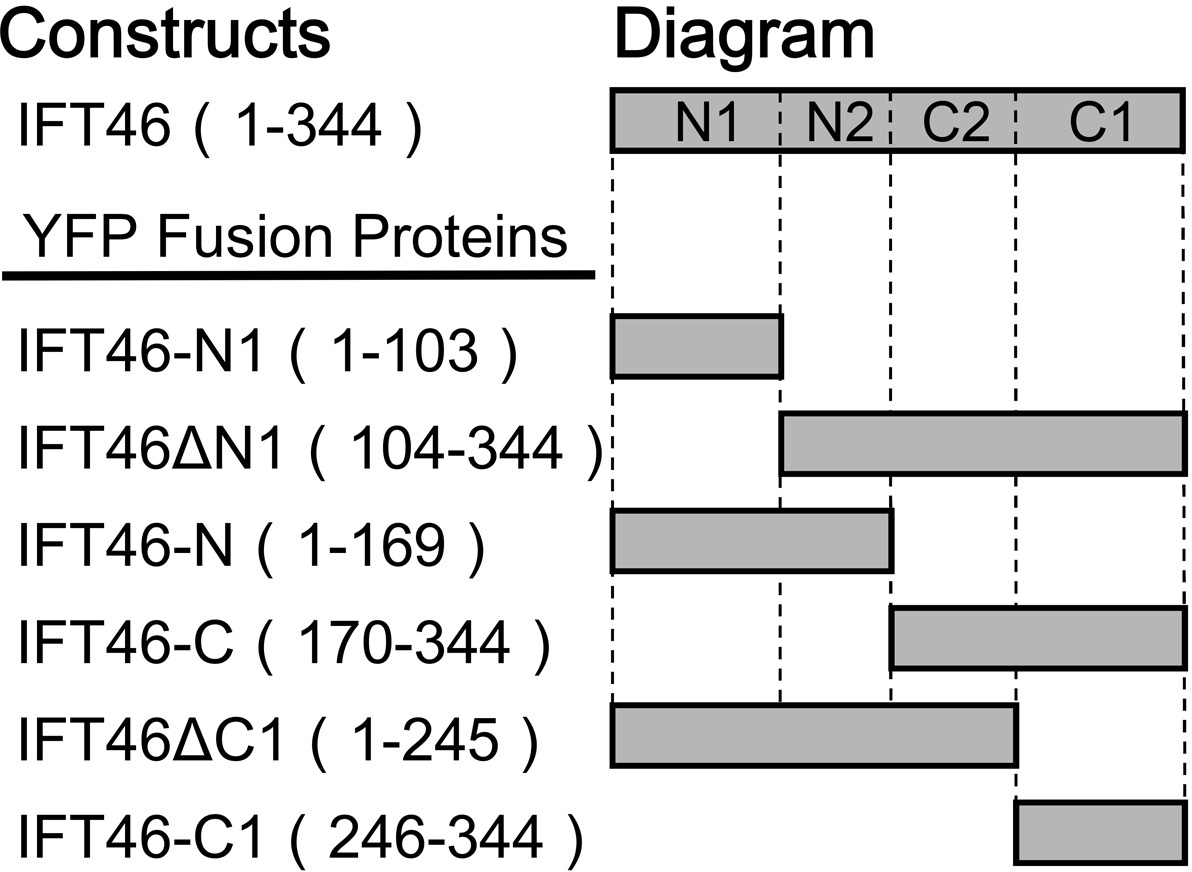
\includegraphics[width=\textwidth-80mm]{fig4-4.jpg}
%生成中英双语标题
{\setstretch{1.667}
\bicaption[fig:4.4]{图}{全长和截短的\ IFT46\ 的示意图。所有片段的\ C\ 端均融合了\textcolor{yellow}{黄色}荧光蛋白。}{Figure}{Diagram of the full-length and the truncated IFT46 produced in this study. YFPs are fused to the C-termini of full-length and the truncated IFT46.}
\par}
%结束图片浮动体环境
\end{figure}

%开始图片浮动体环境,其中!表示取消严谨限制,h表示在此处插入,t表示在本页或下一页顶部插入
\begin{figure}[hbtp!]
%居中对齐
\centering
%设置图片搜索路径,每个路径用{}括起来
\graphicspath{{figures/}}
%插入图片并设置图片宽度为文本宽度减10mm
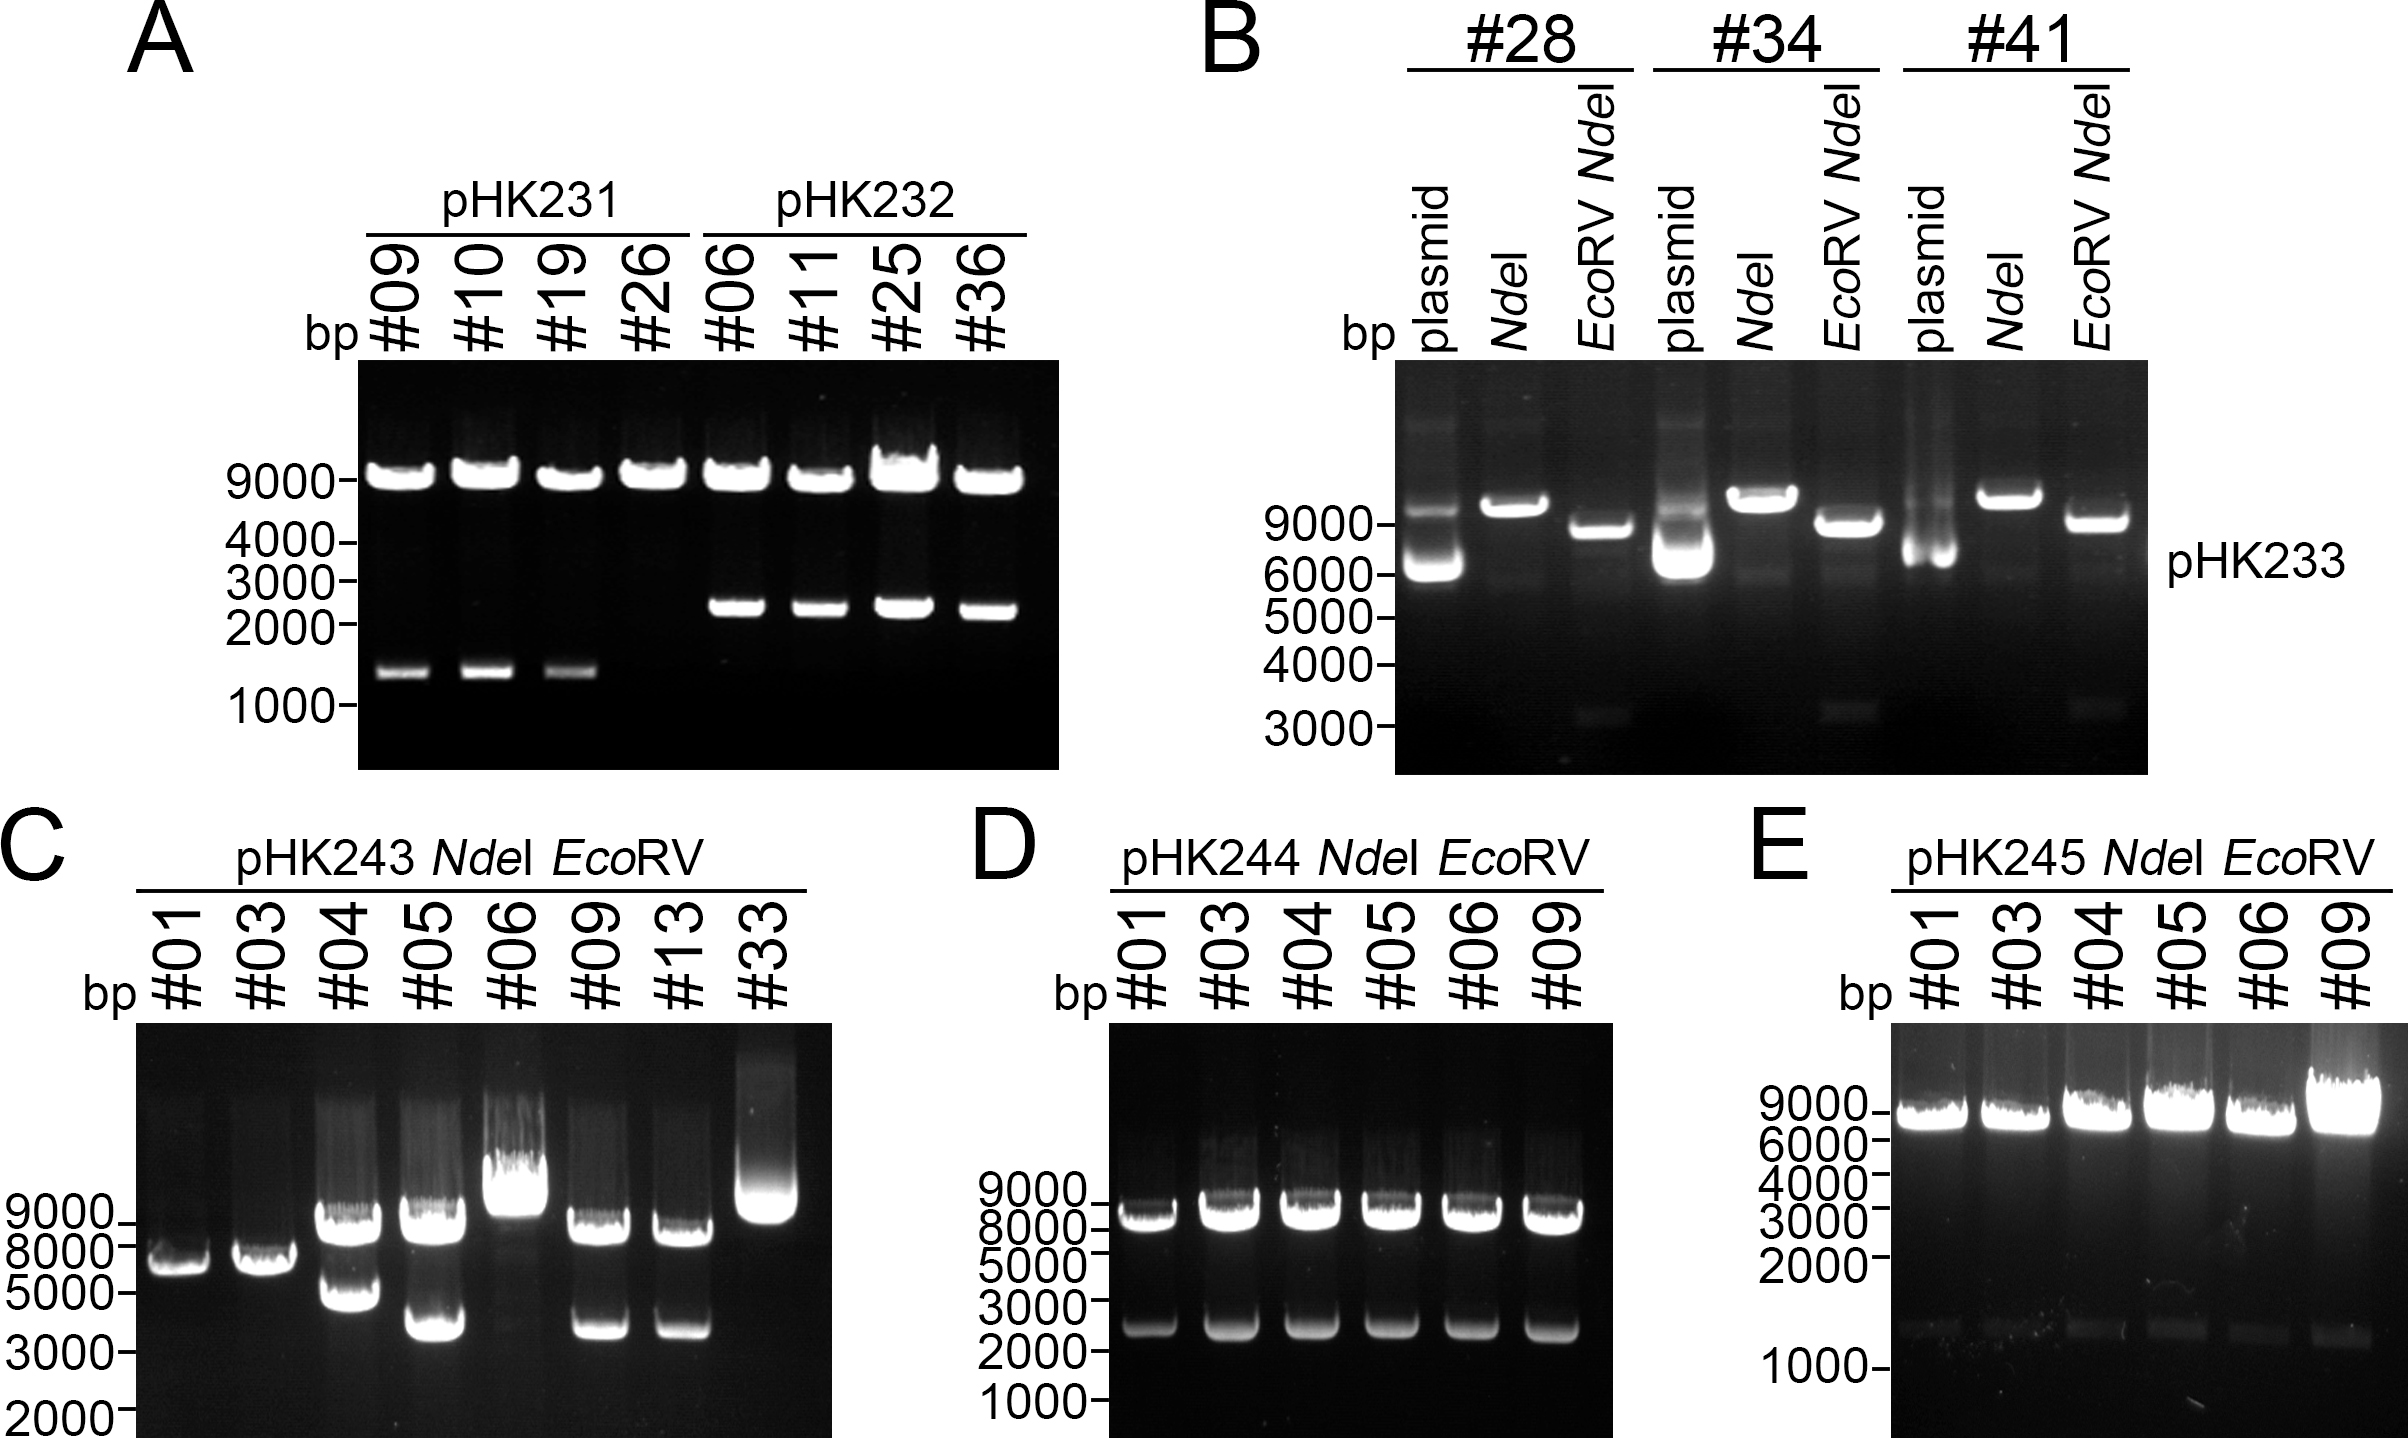
\includegraphics[width=\textwidth-50mm]{fig4-X.jpg}
%生成中英双语标题
{\setstretch{1.667}
\bicaption[fig:4.X]{图}{pHK231、pHK232、pHK233、pHK243、pHK244\ 和\ pHK245\ 酶切产物电泳图。(A)四个\ pHK231\ 及四个\ pHK232\ 疑似阳性克隆酶切后的电泳结果。(B)三个\ pHK233\ 疑似阳性克隆酶切后的电泳结果。(C)八个\ pHK243\ 疑似阳性克隆酶切后的电泳结果。(D)六个\ pHK244\ 疑似阳性克隆酶切后的电泳结果。(E)六个\ pHK245\ 疑似阳性克隆酶切后的电泳结果。所有质粒均用\ \textit{Nde}I\ 和\ \textit{Eco}RV\ 双酶切。这些载体双酶切后目的条带的理论大小依次为\ 1.3 kbp、2.2 kbp、3.2 kbp、3.1 kbp、2.2 kbp\ 和\ 1.3 kbp。} {Figure}{Agarose gel electrophoresis of restriction enzymes-digested pHK231, pHK232, pHK233, pHK243, pHK244, and pHK245. (A) Agarose gel electrophoresis of four suspected positive clones of pHK231 and pHK232. (B) Agarose gel electrophoresis of three suspected positive clones of pHK233. (C) Agarose gel electrophoresis of eight suspected positive clones of pHK243. (D) Agarose gel electrophoresis of six suspected positive clones of pHK244. (E) Agarose gel electrophoresis of six suspected positive clones of pHK245. All plasmids are digested with \textit{Nde}I and \textit{Eco}RV). In theory, the target band sizes of these plasmids are 1.3 kbp, 2.2 kbp, 3.2 kbp, 3.1 kbp, 2.2 kbp and 1.3 kbp, respectively.}
\par}
%结束图片浮动体环境
\end{figure}

%开始图片浮动体环境,其中!表示取消严谨限制,h表示在此处插入,t表示在本页或下一页顶部插入
\begin{figure}[htbp!]
%居中对齐
\centering
%设置图片搜索路径,每个路径用{}括起来
\graphicspath{{figures/}}
%插入图片并设置图片宽度为文本宽度减10mm
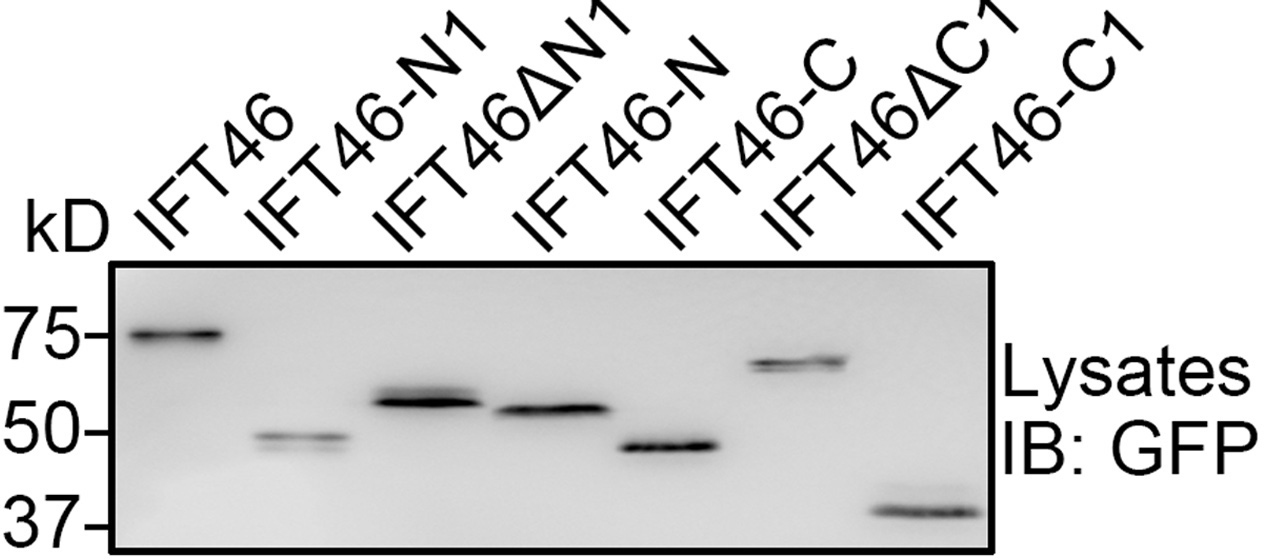
\includegraphics[width=\textwidth-80mm]{fig4-Z.jpg}
%生成中英双语标题
{\setstretch{1.667}
\bicaption[fig:4.Z]{图}{阳性克隆全细胞裂解液免疫印迹分析。IB\ 代表免疫印迹。}{Figure}{Immunoblots of whole-cell lysates (5 $\upmu$g protein per lane) probed with anti-GFP antibody. IB represents immunoblot.}
\par}
%结束图片浮动体环境
\end{figure}

\subsection{构建表达\ IFT46\ 截短片段的载体}
根据前面的分析,我们选定第\ 103、169和245\ 号氨基酸残基为截断位点。为此我们构建了\ pHK231、pHK232、pHK233、pHK
243、pHK244\ 和\ pHK245。这些载体在衣藻中分别表达\ IFT46-N1、IFT46-N、IFT46$\Delta$C1、IFT46$\Delta$N1、IFT46-C\ 和\ IFT46-C1。如图\ \ref{fig:4.X}\ 所示,所有载体均经酶切验证。比如\ pHK231\ 和\ pHK244,目的条带大小分别为\ 1.3 kbp\ 和\ 2.2 kbp。 在实际电泳结果中它们的大小分别在\ 1.3 kbp\ 和\ 2.2 kbp\ 左右。选定酶切大小正确的克隆进行测序验证,没有发生错义突变的克隆即用于后续实验。

\subsection{IFT46-C1\ 是\ IFT46\ 的基体定位序列}
将前面构建的载体转化至\ \textit{ift46-1}\ 中。由于没有任何片段能够拯救或部分拯救\ \textit{ift46-1}\ 的鞭毛缺失表型,我们使用抗\ GFP\ 的抗体通过免疫印迹筛选出阳性克隆。免疫印迹结果显示所有融合蛋白均正常表达且分子量与预期大小一致
(图\ \ref{fig:4.Z})。比如\ IFT46-N::YFP\ 的理论分子量大小为\ 46.3 kDa,免疫印迹结果显示其分子量约\ 50 kDa\ 左右
(图\ \ref{fig:4.Z} 泳道\ 4)。

接下来我们利用激光共聚焦显微镜观察了\ IFT46\ 的截短片段在细胞体中的定位。融合蛋白\ IFT46-N1::YFP、IFT46-N::YFP\ 和\ IFT46$\Delta$C1::YFP\ 没有聚集在基体周围而是在细胞体中均匀分布(
图\ \ref{fig:4.6}A)。然而,IFT46$\Delta$N1::YFP、IFT46-C::YFP\ 和\ IFT46-C1\ 确能够继续定位在基体(图\ \ref{fig:4.6}A)。由于\ IFT46$\Delta$N1::YFP、IFT46-C::YFP\ 和\ IFT46-C1\ 均含有\ C1\ 结构域,这表明\ C1\ 结构域是\ IFT46\ 的基体定位序列。

%开始图片浮动体环境,其中!表示取消严谨限制,h表示在此处插入,t表示在本页或下一页顶部插入
\begin{figure}[h!btp]
%居中对齐
\centering
%设置图片搜索路径,每个路径用{}括起来
\graphicspath{{figures/}}
%插入图片并设置图片宽度为文本宽度减10mm
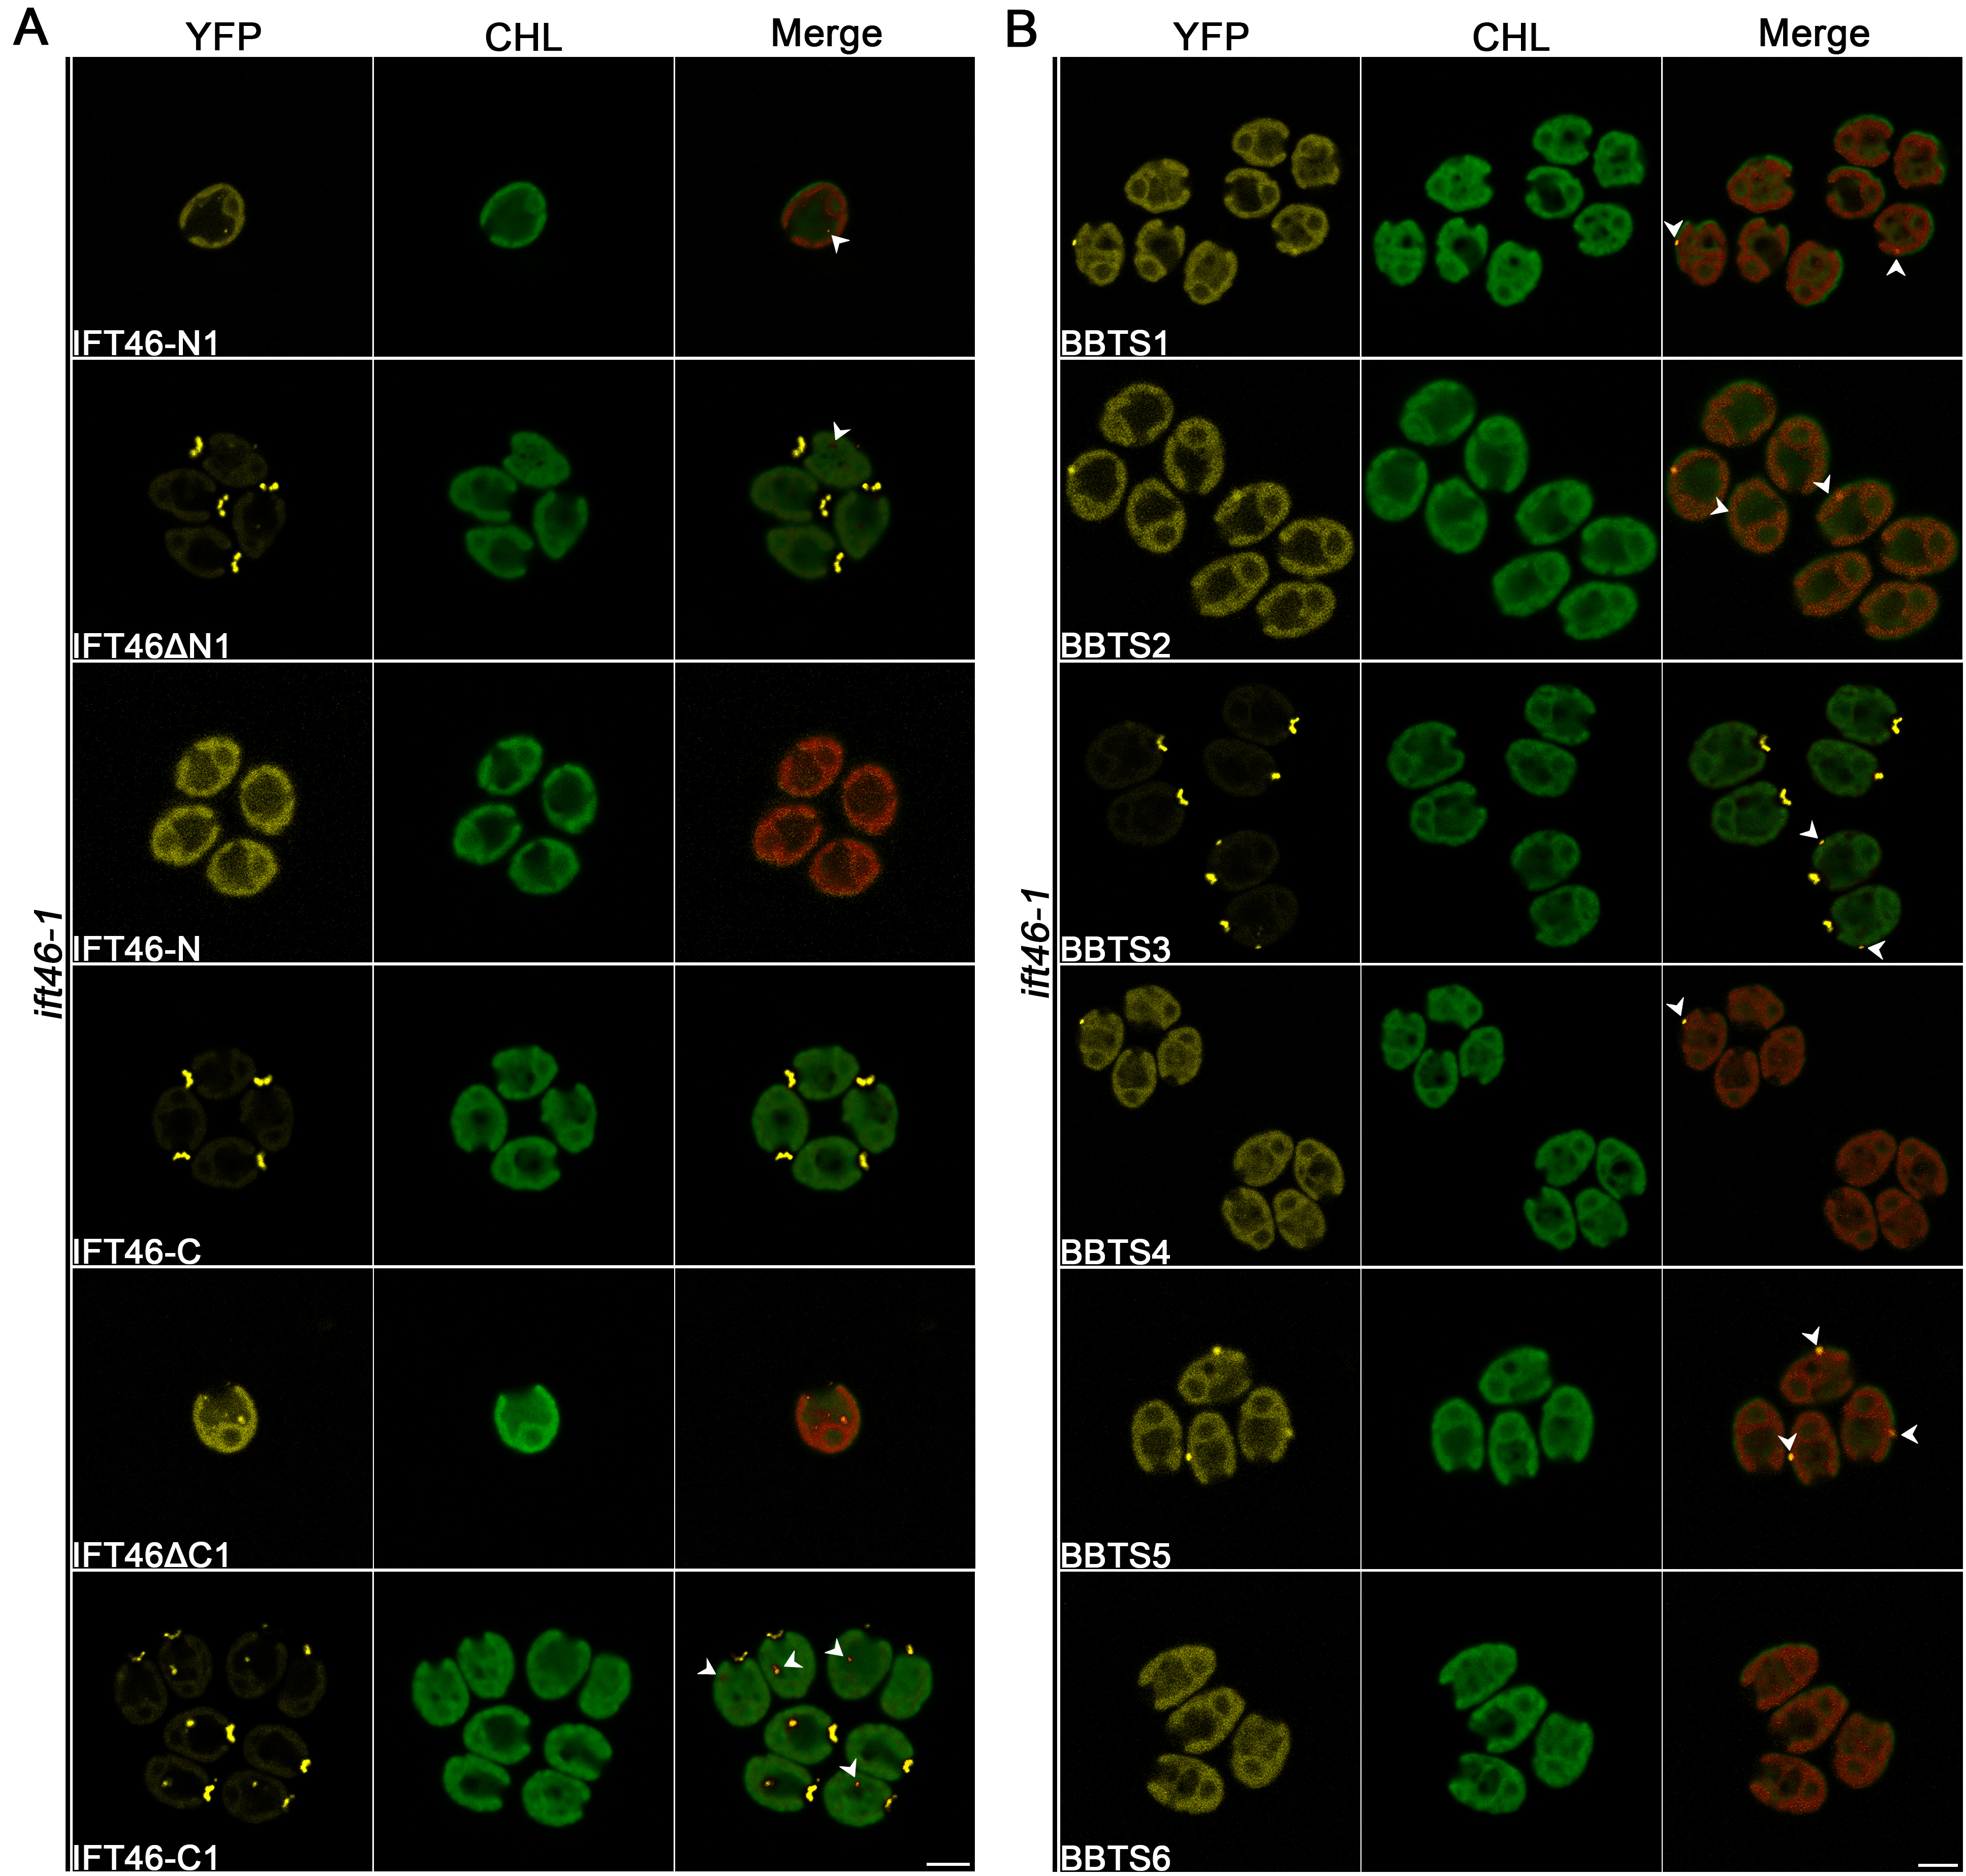
\includegraphics[width=\textwidth]{fig4-6.jpg}
%生成中英双语标题
{\setstretch{1.667}
\bicaption[fig:4.6]{图}{IFT46-C1\ 和\ BBTS3\ 是\ IFT46\ 的基体定位序列。(A)表达IFT46-N1::YFP、IFT46$\Updelta$N1::YFP、IFT46-N::YFP、IFT46-C::YFP、IFT46$\Updelta$C1::YFP\ 或\ IFT46-C1::YFP\ 的\
\textit{ift46-1}\ 藻株的共聚焦成像结果。其中\ IFT46$\Updelta$N1::YFP、IFT46-C::YFP\ 和\ IFT46-C1::YFP\ 可定位在基体。(B)表达\ BBTS1::YFP、BBTS2::YFP、BBTS3::YFP、BBTS4::YFP、BBTS5::YFP\ 或\ BBTS6::YFP\ 的\ \textit{ift46-1}\ 藻株的共聚焦成像结果。仅\ BBTS3::YFP\ 可定位在基体。在\ A\ 和\ B\ 中,白色箭头代表眼点,CHL\ 代表叶绿素,标尺代表\ \ \SI{5}{\um}。}{Figure}{IFT46-C1 and BBTS3 are the basal body targeting sequences of IFT46. (A) Confocal imaging of \textit{ift46-1} expressing IFT46-N1::YFP, IFT46$\Updelta$N1::YFP, IFT46-N::YFP, IFT46-C::YFP, IFT46$\Updelta$C1::YFP or IFT46-C1::YFP separately. IFT46$\Updelta$N1::YFP, IFT46-C::YFP, and IFT46-C1::YFP are able to localize at basal bodies. (B) Confocal imaging of \textit{ift46-1} expressing BBTS1::YFP, BBTS2::YFP, BBTS3::YFP, BBTS4::YFP, BBTS5::YFP or BBTS6::YFP separately. Only BBTS3::YFP is able to localize at basal bodies. In panel A and B, White arrows: eyespots; CHL: chlorophyll; Scale bars represent 5 $\upmu$m.}
\par}
%结束图片浮动体环境
\end{figure}

%开始图片浮动体环境,其中!表示取消严谨限制,h表示在此处插入,t表示在本页或下一页顶部插入
\begin{figure}[!ht]
%居中对齐
\centering
%设置图片搜索路径,每个路径用{}括起来
\graphicspath{{figures/}}
%插入图片并设置图片宽度为文本宽度减10mm
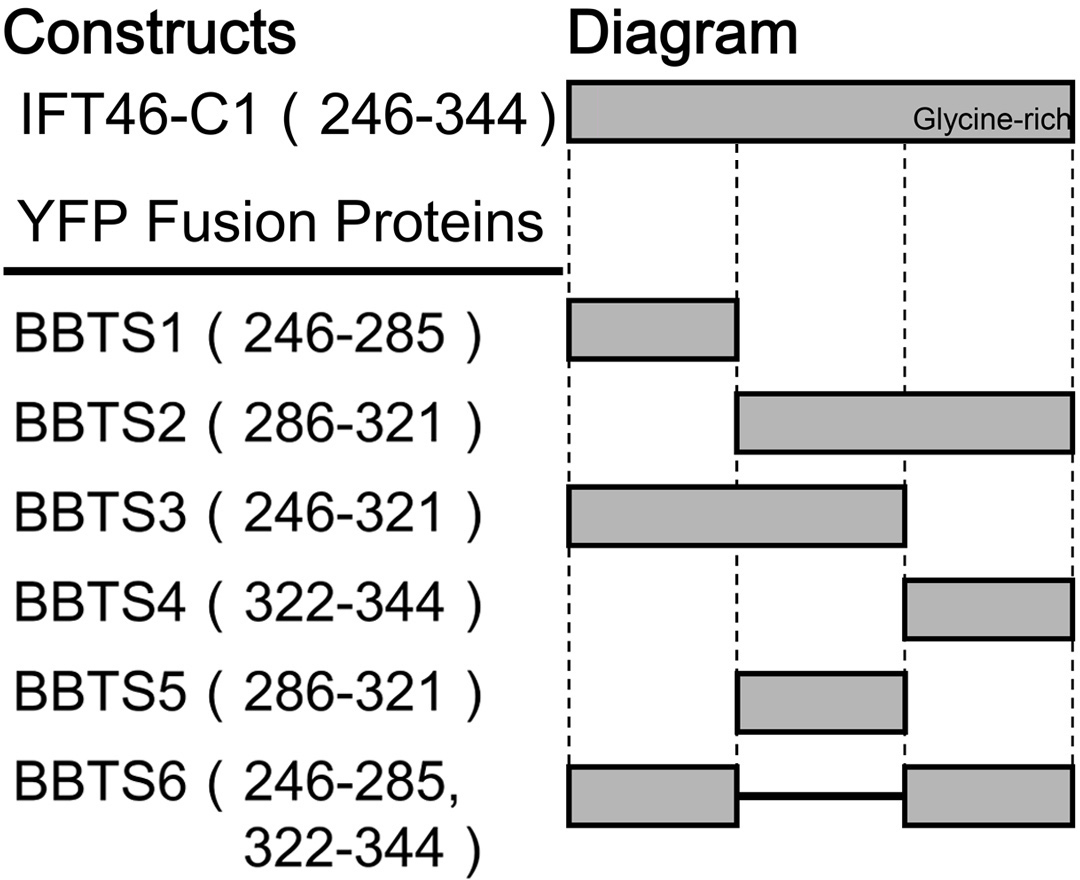
\includegraphics[width=\textwidth-80mm]{fig4-5.jpg}
%生成中英双语标题
{\setstretch{1.667}
\bicaption[fig:4.5]{图}{全长和截短的\ IFT46-C1\ 的示意图。所有片段的\ C\ 端均融合了\textcolor{yellow}{黄色}荧光蛋白。}{Figure}{Diagram of the full-length and the truncated IFT46-C1 produced in this study. YFPs are fused to the C-termini of full-length and the truncated IFT46-C1.}
\par}
%结束图片浮动体环境
\end{figure}

%开始图片浮动体环境,其中!表示取消严谨限制,h表示在此处插入,t表示在本页或下一页顶部插入
\begin{figure}[h!tbp]
%居中对齐
\centering
%设置图片搜索路径,每个路径用{}括起来
\graphicspath{{figures/}}
%插入图片并设置图片宽度为文本宽度减10mm
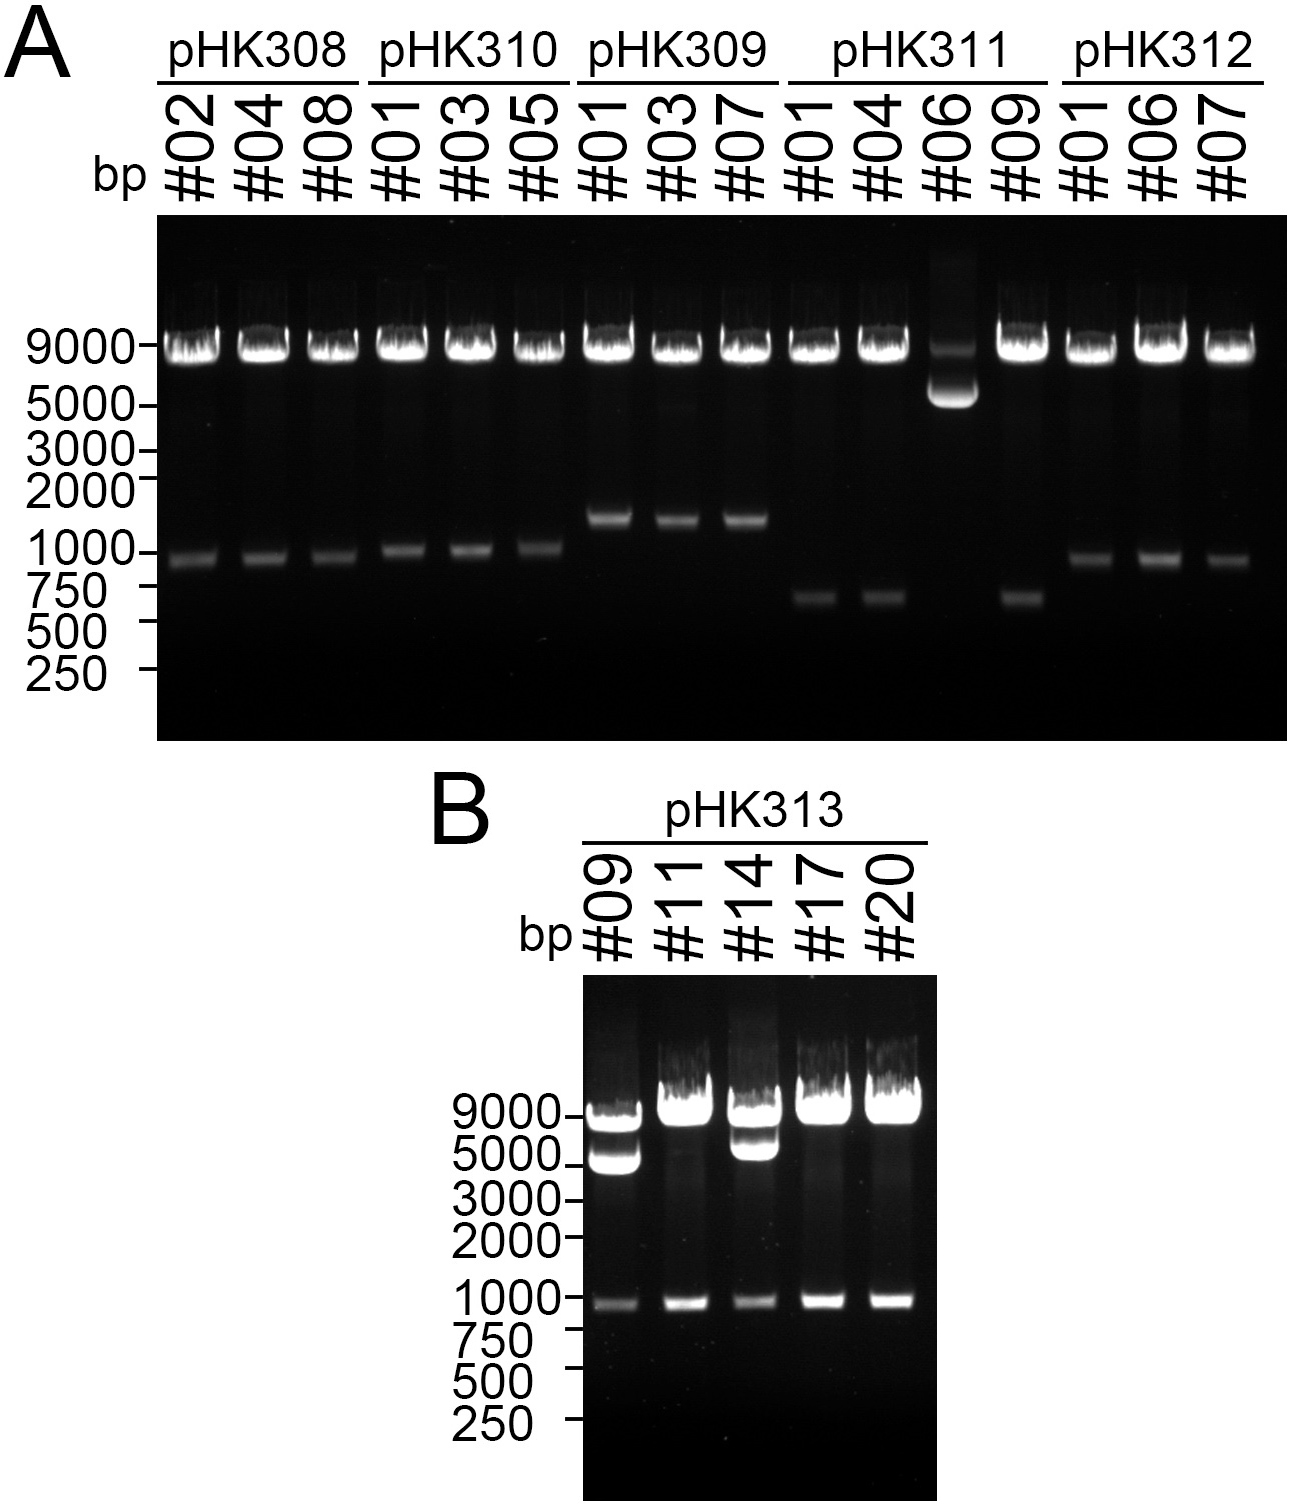
\includegraphics[width=\textwidth-70mm]{fig4-Y.jpg}
%生成中英双语标题
{\setstretch{1.667}
\bicaption[fig:4.Y]{图}{pHK308、pHK310、pHK309、pHK311、pHK312\ 和\ pHK313\ 酶切产物电泳图。(A)三个\ pHK308(\#02、\#04\ 和\ \#08),三个\ pHK310(\#01、\#03\ 和\ \#05),三个\ pHK309(\#01、\#03\ 和\ \#07),四个\ pHK311(\#01、\#04、\#06\ 和\ \#09)\ 以及三个\ pHK312(\#01、\#06\ 和\ \#07)\ 疑似阳性克隆
经\ \textit{Nde}I、\textit{Eco}RV\ 酶切后的电泳结果。这些载体双酶切后目的条带的理论大小依次为\ 850 bp、900 bp、1200 bp、550 bp\ 和\ 830 bp。其中\ pHK311\ 的\ \#06\ 号克隆为阴性,其余所有克隆均为阳性。(B)五个\ pHK313
(\#09、\#11、\#14、\#17\ 和\ \#20)\ 疑似阳性克隆经\ \textit{Nde}I、\textit{Eco}RV\ 酶切后的电泳结果。其目的条带理论大小为\ 900 bp。结果显示\ \#11、\#17\ 和\ \#20\ 号克隆为阳性。在\ A\ 和\ B\ 中,电泳图左侧的数字代表\ DNA marker\ 的大小。}{Figure}{Agarose gel electrophoresis of restriction enzymes-digested pHK308, pHK310, pHK309, pHK311, pHK312, and pHK313. (A) Agarose gel electrophoresis of suspected positive clones of pHK308 (Clone \#02, \#04, and \#08), pHK310 (Clone \#01, \#03, and \#05), pHK309 (Clone \#01, \#03, and \#07), pHK311 (Clone \#01, \#04, \#06, and \#09) and pHK312 (Clone \#01, \#06, and \#07) (digested with \textit{Nde}I and \textit{Eco}RV). In theory, the target band sizes of these vectors are 850 bp, 900 bp, 1200 bp, 550 bp and 830 bp, respectively. Clone \#06 of pHK311 is negative and all other clones are positive according to the band sizes. (B) Agarose gel electrophoresis of five suspected positive clones of pHK313 (Clone \#09, \#11, \#14, \#17, and \#20) (digested with \textit{Nde}I and/or \textit{Eco}RV). The target band size is 900 bp. Clone \#11, \#17, and \#20 of pHK313 are positive according to the band sizes. In panel A and B, numbers on the left sides of the maps represent the ladders of the DNA markers.}
\par}
%结束图片浮动体环境
\end{figure}

\subsection{构建表达\ IFT46-C1\ 截短片段的载体}
由于绝大多数已知的定位序列均比\ IFT46-C1(99个氨基酸残基)短\
\citep{Malicki2014,Bhogaraju2013,McIntyre2015,Dishinger2010,Berbari2008,Hurd2011,Santos2014},我们进一步将\ IFT46-C1\ 截短为六个片段(图\ \ref{fig:4.5})。为此我们构建了\ pHK308、pHK310、pHK309、pHK311、pHK312\ 和\ pHK313。 这些载体在衣藻中分别表达\ BBTS1、BBTS2、BBTS3、BBTS4、BBTS5、 和\ BBTS6。如
图\ \ref{fig:4.Y}\ 所示,所有载体均经酶切验证。比如\ pHK308\ 和\ pHK313,目的条带大小分别约为\ 850 bp\ 和\ 900 bp。 在实际电泳结果中它们的大小在\ 800-900 bp\ 之间。选定酶切大小正确的克隆进行测序验证,没有发生错义突变的克隆即用于后续实验。

\subsection{BBTS3\ 是\ IFT46\ 的基体定位序列}
%开始图片浮动体环境,其中!表示取消严谨限制,h表示在此处插入,t表示在本页或下一页顶部插入
\begin{figure}[!ht]
%居中对齐
\centering
%设置图片搜索路径,每个路径用{}括起来
\graphicspath{{figures/}}
%插入图片并设置图片宽度为文本宽度减10mm
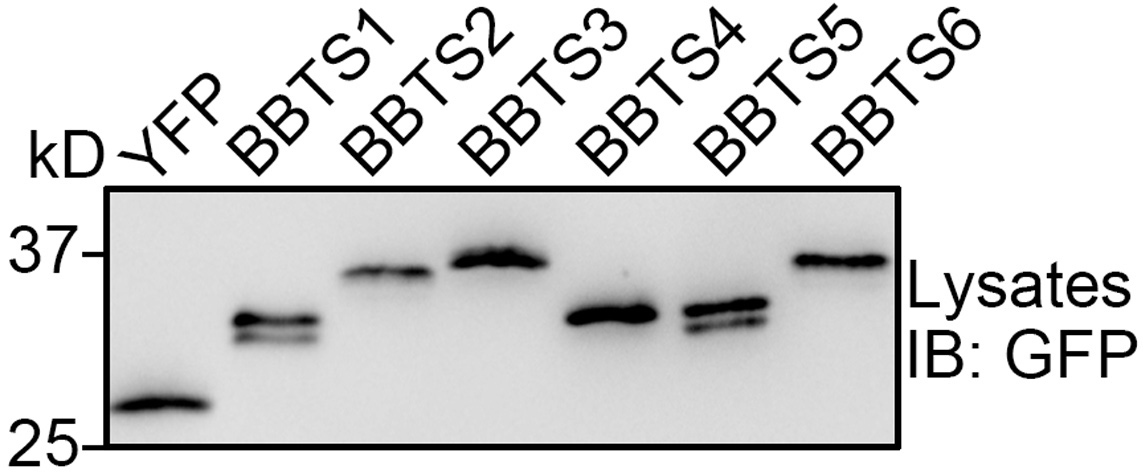
\includegraphics[width=\textwidth-80mm]{fig4-K.jpg}
%生成中英双语标题
{\setstretch{1.667}
\bicaption[fig:4.K]{图}{阳性克隆全细胞裂解液免疫印迹分析。IB\ 代表免疫印迹。}{Figure}{Immunoblots of whole-cell lysates (5 $\upmu$g protein per lane) probed with anti-GFP antibody. IB represents immunoblot.}
\par}
%结束图片浮动体环境
\end{figure}

将前面构建的载体转化至\ \textit{ift46-1}\ 中,使用抗\ GFP\ 的抗体通过免疫印迹筛选出阳性克隆(
图\ \ref{fig:4.K})。免疫印迹结果显示所有融合蛋白均正常表达且分子量与预期大小一致(
图\ \ref{fig:4.K})。取阳性克隆进行活细胞成像,结果显示\ BBTS1::YFP、BBTS2::YFP、BBTS4::YFP、 BBTS5::YFP\ 和\ BBTS6::YFP\ 均无法继续定位在基体(图\ \ref{fig:4.6}B),而\ BBTS3::YFP\ 可继续在基体附近聚集(图\ \ref{fig:4.6}B)。这些结果表明\ BBTS3(76\ 个氨基酸残基)是我们目前鉴定到的最短的\ IFT46\ 的基体定位序列。

\subsection{IFT46-C1/BBTS3\ 是\ IFT46\ 的纤毛定位序列}
%开始图片浮动体环境,其中!表示取消严谨限制,h表示在此处插入,t表示在本页或下一页顶部插入
\begin{figure}[!ht]
%居中对齐
\centering
%设置图片搜索路径,每个路径用{}括起来
\graphicspath{{figures/}}
%插入图片并设置图片宽度为文本宽度减10mm
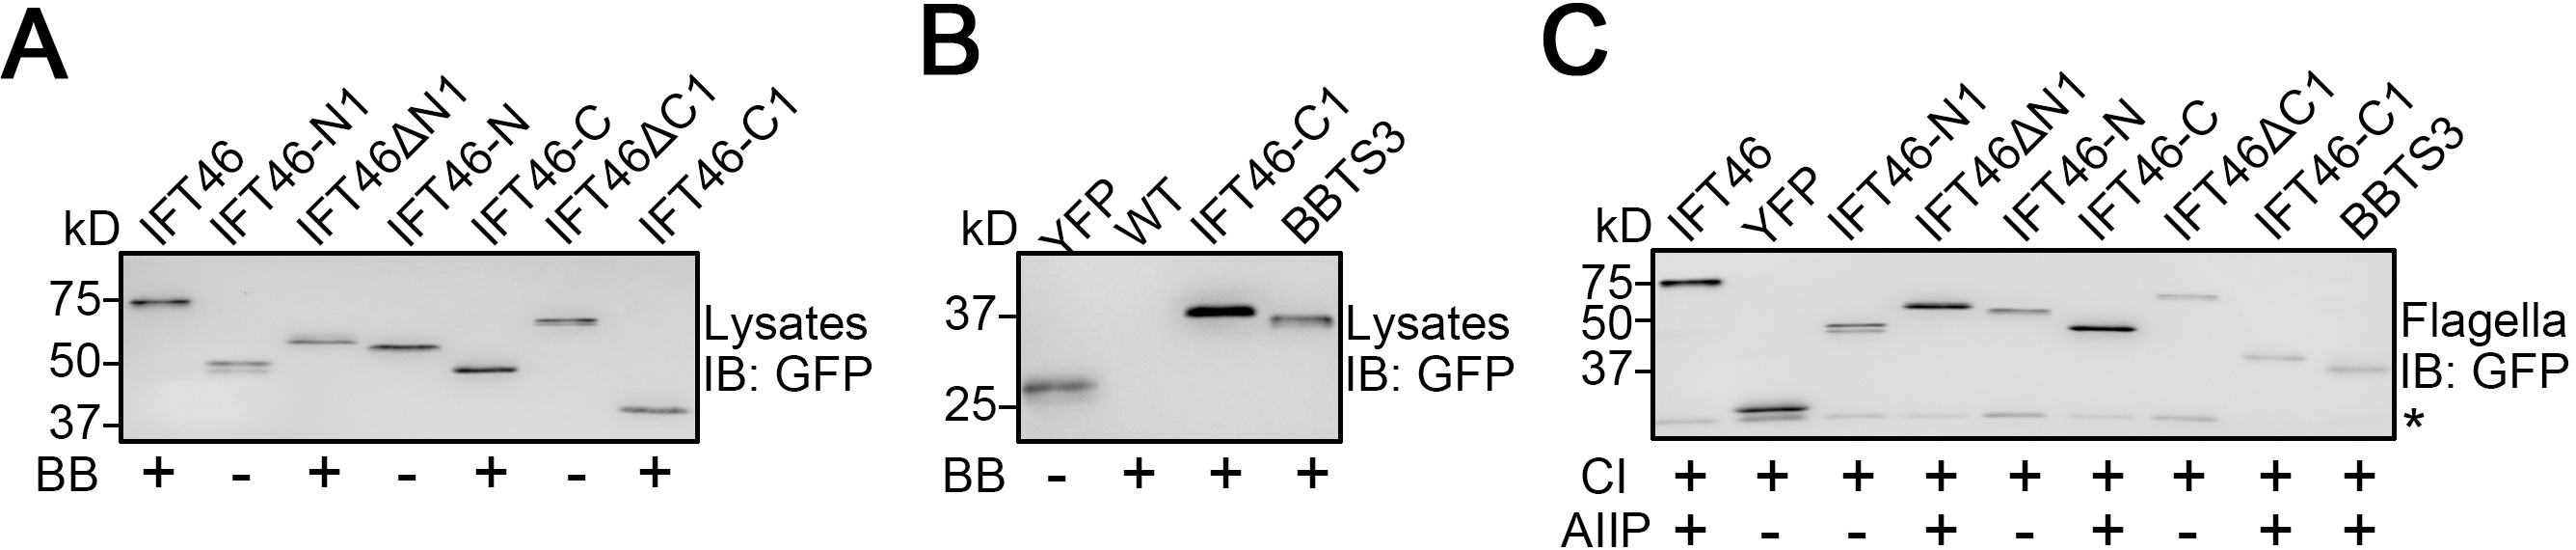
\includegraphics[width=\textwidth]{fig4-7.jpg}
%生成中英双语标题
{\setstretch{1.667}
\bicaption[fig:4.7]{图}{在\ CC-125\ 中表达\ IFT46\ 的截短片段。(A,B)阳性克隆全细胞裂解液免疫印迹分析。WT\ 代表野生型\ CC-125\ 细胞。BB\ 代表基体。加号代表对应的蛋白定位在基体,减号则相反。(C)阳性克隆鞭毛膜/基质免疫印迹分析。CI\ 代表纤毛,AIIP\ 代表蛋白组装在\ IFT\ 复合物中。加号代表对应的蛋白能够进入纤毛且组装在\ IFT\ 复合物中。减号则相反。IB\ 代表免疫印迹。}{Figure}{Expression of truncated IFT46 in CC-125. (A, B) Immunoblots of whole-cell lysates (5 $\upmu$g protein per lane) of CC-125 expressing indicated proteins probed with the anti-GFP antibody. WT: WT CC-125 cells; BB: the basal body. Plus signs mean the corresponding proteins localize in the basal body region. While minus signs indicate not. IB: immunoblot. (C) Immunoblot of flagellar membrane-plus-matrix fractions of CC-125 expressing indicated proteins probed with the indicated antibodies. CI: cilia; AIIP: assembled in IFT particles. Plus signs mean the corresponding proteins entered into cilia and assembled in IFT particle. While minus signs indicate not. IB: immunoblot.}
\par}
%结束图片浮动体环境
\end{figure}

前面我们发现\ IFT46-C1\ 和\ BBTS3\ 是\ IFT46\ 的基体定位序列(图\ \ref{fig:4.8})。接下来的问题是它们是否也是\ IFT46\ 的纤毛定位序列。为了阐明这个问题,我们将全长\ IFT46\ 和\ IFT46\ 的截短片段表达在野生型\ CC-125\ 细胞中。利用抗\ GFP\ 的抗体我们通过免疫印迹筛选出阳性克隆
(图\ \ref{fig:4.7}A)。结果显示所有融合蛋白均正常表达且分子量与预期大小一致(图\ \ref{fig:4.7}A)。利用共聚焦成像,我们观察了这些融合蛋白的亚细胞定位。结果显示\ IFT46::YFP、IFT46$\Delta$N1::YFP、IFT46-C::YFP\ 和\ IFT46-C1::YFP\ 主要定位在基体和鞭毛
(图\ \ref{fig:4.8}A)。然而,与在\ \textit{ift46-1}\ 中的结果一致,IFT46-N1::YFP、 IFT46-N::YFP\ 和\ IFT46$\Delta$C1::YFP\ 无法定位在基体(图\ \ref{fig:4.8}A)。有意思的是,通过免疫印迹我们能够在鞭毛中检测到所有的融合蛋白(图\ \ref{fig:4.7}C)。由于共聚焦显微镜可能无法观察到鞭毛中微弱的荧光信号,我们借助全内反射荧光显微镜发现鞭毛中确实存在\ IFT46-N1::YFP、 IFT46-N::YFP\ 和\ IFT46$\Delta$C1::YFP\ 的微弱信号(图\ \ref{fig:4.8}C)。这些荧光信号均匀分布且无法移动。由于这三个融合蛋白的分子量均小于\ 100 kDa,它们极有可能是通过自由扩散穿越转变区进入纤毛的\
\citep{Hu2010,Chih2011,Kee2012,Breslow2013}。以上结果再次说明\ IFT46-C1\ 是\ IFT46\ 的基体定位序列,同时也表明\ IFT46-C1\ 是\ IFT46\ 的纤毛定位序列。

%开始图片浮动体环境,其中!表示取消严谨限制,h表示在此处插入,t表示在本页或下一页顶部插入
\begin{figure}[htbp]
%居中对齐
\centering
%设置图片搜索路径,每个路径用{}括起来
\graphicspath{{figures/}}
%插入图片并设置图片宽度为文本宽度减10mm
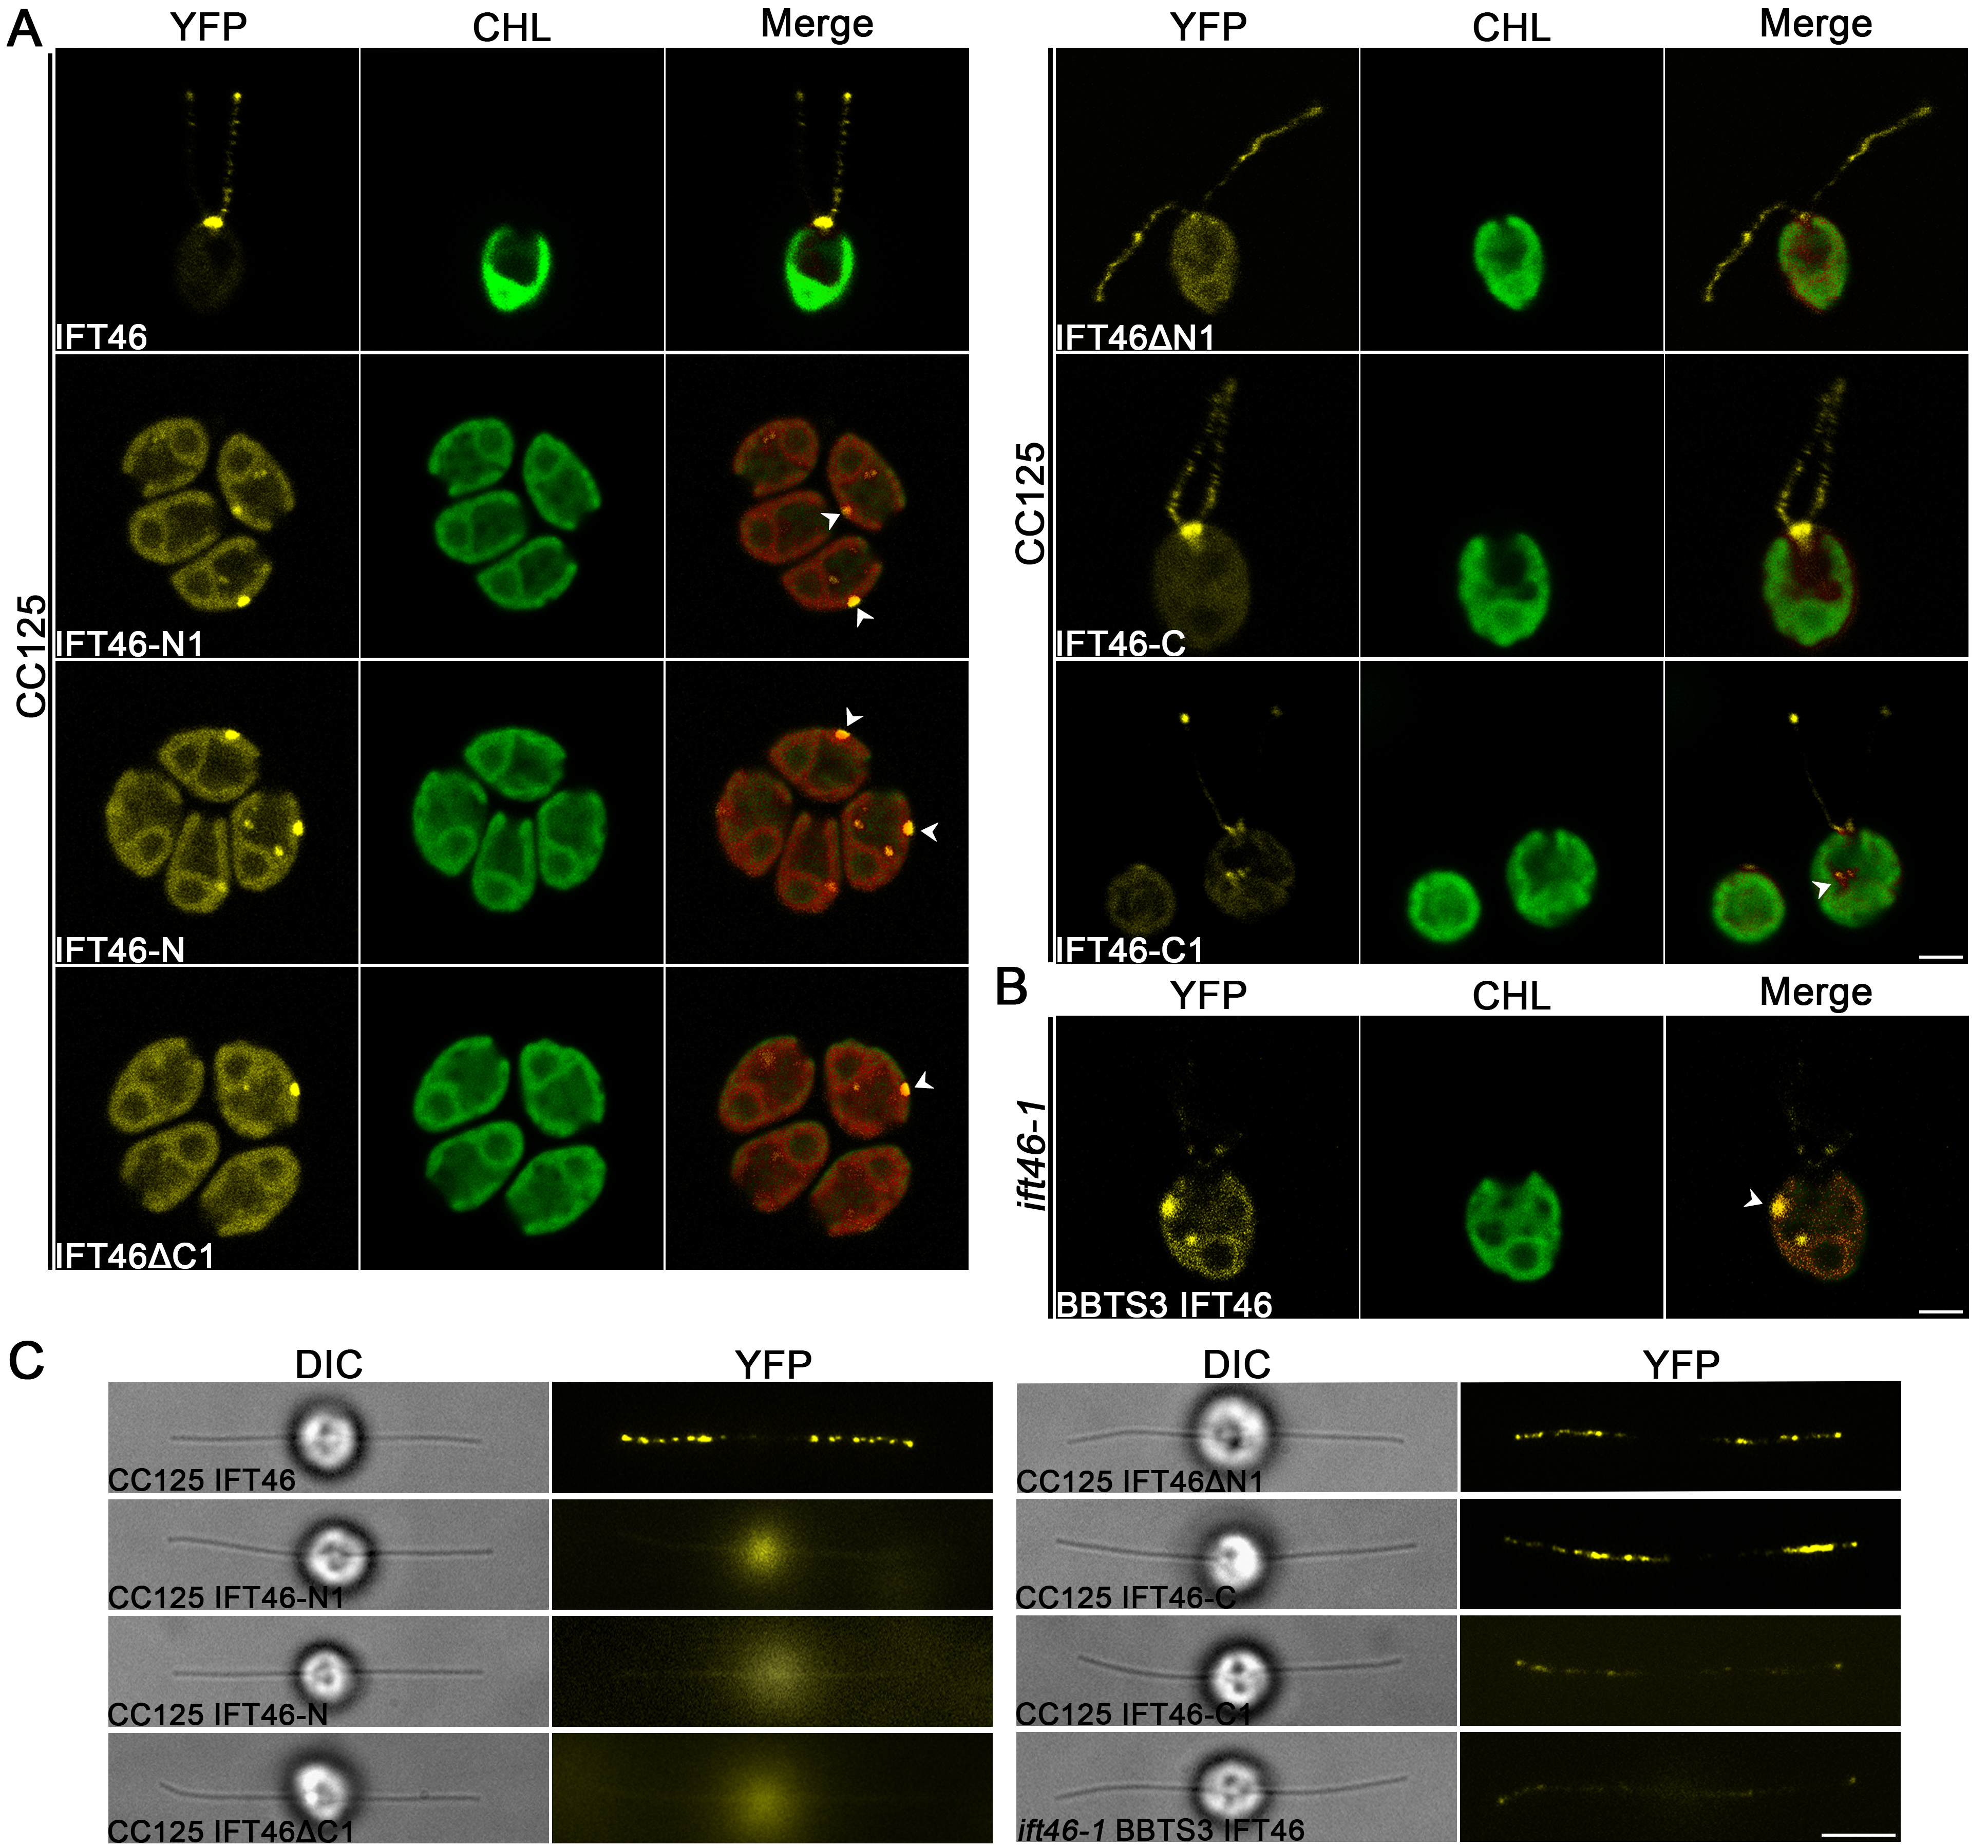
\includegraphics[width=\textwidth]{fig4-8.jpg}
%生成中英双语标题
{\setstretch{1.667}
\bicaption[fig:4.8]{图}{IFT46-C1\ 和\ BBTS3\ 是\ IFT46\ 的纤毛定位序列。(A)表达\ IFT46::YFP、IFT46-N1::YFP、 IFT46$\Delta$N1::YFP、IFT46-N::YFP、IFT46-C::YFP、IFT46$\Delta$C1::YFP\ 或\ IFT46-C1::YFP\ 的\ CC-125\ 藻株的共聚焦成像结果。(B)表达\ BBTS3::YFP\ 和\ IFT46\ 的\ \textit{ift46-1}\ 藻株的共聚焦成像结果。在\ A\ 和\ B\ 中白色箭头代表眼点。(C)A\ 和\ B\ 中藻株的鞭毛的全内反射荧光显微成像结果。左侧为微分干涉成像图片。在\ A-C\ 中,标尺代表\ \SI{5}{\um}。}{Figure}{IFT46-C1 and BBTS3 are the ciliary targeting sequences of IFT46. (A) Confocal imaging of CC-125 expressing IFT46::YFP, IFT46-N1::YFP, IFT46$\Delta$N1::YFP, IFT46-N::YFP, IFT46-C::YFP, IFT46$\Delta$C1::YFP, IFT46-C1::YFP separately. White arrows: eyespots; CHL: chlorophyll. (B) Confocal imaging of \textit{ift46-1} expressing BBTS3::YFP and IFT46. White arrows: eyespots; CHL: chlorophyll. (C) TIRFM imaging of the flagella of the strains listed in A and B. Differential interference contrast images are shown on the left. CHL: chlorophyll. In panel A-C, scale bars represent 5 $\upmu$m.}
\par}
%结束图片浮动体环境
\end{figure}

由于\ BBTS3\ 是我们目前鉴定到的最短的\ IFT46\ 的基体定位序列,我们希望知道\ BBTS3\ 是否也是\ IFT46\ 的纤毛定位序列。然而,将\ pHK309\ 转化至野生型\ CC-125\ 细胞中,我们筛选了两百个转化子未能获得阳性克隆。这可能是由于\ BBTS3\ 在\ CC-125\ 中表达量低或不稳定造成的。由于我们能够获得\
\textit{ift46-1}\ \textit{BBTS3},我们将\ \textit{IFT46}\ 的基因组\ DNA\ 和\ pHyg3\ 共转化至
\textit{ift46-1}\ \textit{BBTS3}\ 从而得到\ \textit{ift46-1}\ \textit{BBTS3::YFP IFT46}(
图\ \ref{fig:4.7}B)。 理论上,
\textit{ift46-1}\ \textit{BBTS3::YFP IFT46}\ 与\ CC-125 \textit{BBTS3}\ 相当。共聚焦和全内反射荧光显微成像结果显示\ BBTS3\ 定位在基体和鞭毛且能够沿鞭毛作双向运动(图\ \ref{fig:4.8}B, C)。总之,BBTS3\ 是\ IFT46\ 中已知最短的纤毛定位序列。

与\ IFT46-C1\ 相比,BBTS3\ 缺少\ C\ 端的甘氨酸尾巴,这段富含甘氨酸的肽段在其他物种的\ IFT46\ 中并不存在(图\ \ref{fig:4.10})。 通过免疫印迹分析我们发现在有全长\ IFT46\ 存在的情况下,IFT46-C1\ 的表达水平下降至\ 30\% (图\ \ref{fig:4.9}A, B)。在有全长\ IFT46\ 存在的情况下,BBTS3\ 的表达水平与IFT46-C1\ 相当(图\ \ref{fig:4.9}C, D)。然而,相比于\ IFT46-C1,BBTS3\ 在全长\ IFT46\ 存在的情况下稳定性更差。在阳性克隆传代的过程中该蛋白更容易丢失或沉默。这表明莱茵衣藻\ IFT46\ 中的甘氨酸尾巴可能有助于提高其稳定性。由于这一原因,我们选用\ IFT46-C1\ 进行后续实验。

\subsection{IFT46-C1\ 与其他\ IFT-B\ 亚基相互作用}
%开始图片浮动体环境,其中!表示取消严谨限制,h表示在此处插入,t表示在本页或下一页顶部插入
\begin{figure}[htbp]
%居中对齐
\centering
%设置图片搜索路径,每个路径用{}括起来
\graphicspath{{figures/}}
%插入图片并设置图片宽度为文本宽度减10mm
\includegraphics[width=\textwidth]{fig4-10.jpg}
%生成中英双语标题
{\setstretch{1.667}
\bicaption[fig:4.10]{图}{IFT46-C1\ 在进化上高度保守。来自不同物种(衣藻、团藻、智人、小鼠、秀丽隐杆线虫、爪蟾、黄牛、家犬、大鼠、鸡、斑马鱼、紫海胆、日本血吸虫、球石藻(颗石藻)、嗜热四膜虫以及蜜蜂)的\ IFT46-C1\ 的多重序列比对结果显示\ IFT46\ 的\ C\ 端在进化上高度保守。黑色三角形代表选定的用于定点突变的两个亮氨酸残基。黑色正方形代表衣藻\ IFT46\ 特有的富含甘氨酸的尾巴。一致序列和代表保守程度的图形显示在序列下方。}{Figure}{IFT46-C1 is highly conserved in evolution. The amino acid sequences of IFT46-C1 from \textit{Chlamydomonas reinhardtii}, \textit{Volvox carteri f. nagariensis}, \textit{Homo sapiens}, \textit{Mus musculus}, \textit{Caenorhabditis elegans}, \textit{Xenopus laevis}, \textit{Bos taurus}, \textit{Canis lupus familiaris}, \textit{Rattus norvegicus}, \textit{Gallus gallus}, \textit{Danio rerio}, \textit{Strongylocentrotus purpuratus}, \textit{Schistosoma japonicum}, \textit{Emiliania huxleyi CCMP1516}, \textit{Tetrahymena thermophila}, and \textit{Apis mellifera} were aligned. The black triangles mark the two critical hydrophobic leucines we chosen for mutagenesis. The black squares mark the glycine-rich tail of CrIFT46. The consensus sequence and the graph showing percentages of conservation are given at the bottom.}
\par}
%结束图片浮动体环境
\end{figure}

IFT46-C1\ 和\ BBTS3\ 能够进入鞭毛且沿轴丝双向运动,这表明它们可能与全长\ IFT46\ 一样能够组装到\ IFT-B\ 复合物中\
\citep{Lucker2005,Lucker2010,Taschner2014,Taschner2011,Fan2010}。为了证实这一点,我们分离了\ CC-125 \textit{IFT46-C1::YFP}\ 的鞭毛并获得其鞭毛膜/基质部分。通过免疫共沉淀实验我们发现,与全长\ IFT46\ 一样,IFT46-C1\ 能够与\ IFT81、IFT74/72\ 和\ IFT52\ 形成复合物(图\ \ref{fig:4.11}A)。 蔗糖密度梯度离心的结果也显示\ IFT46-C1\ 能够与\ IFT-B\ 复合物中的\ IFT81\ 形成复合物(图\ \ref{fig:4.11}B)。 以上结果表明\ IFT46-C1\ 能够通过与其他\ IFT-B\ 亚基互作组装到\ IFT-B\ 复合物中。


%开始图片浮动体环境,其中!表示取消严谨限制,h表示在此处插入,t表示在本页或下一页顶部插入
\begin{figure}[htbp]
%居中对齐
\centering
%设置图片搜索路径,每个路径用{}括起来
\graphicspath{{figures/}}
%插入图片并设置图片宽度为文本宽度减10mm
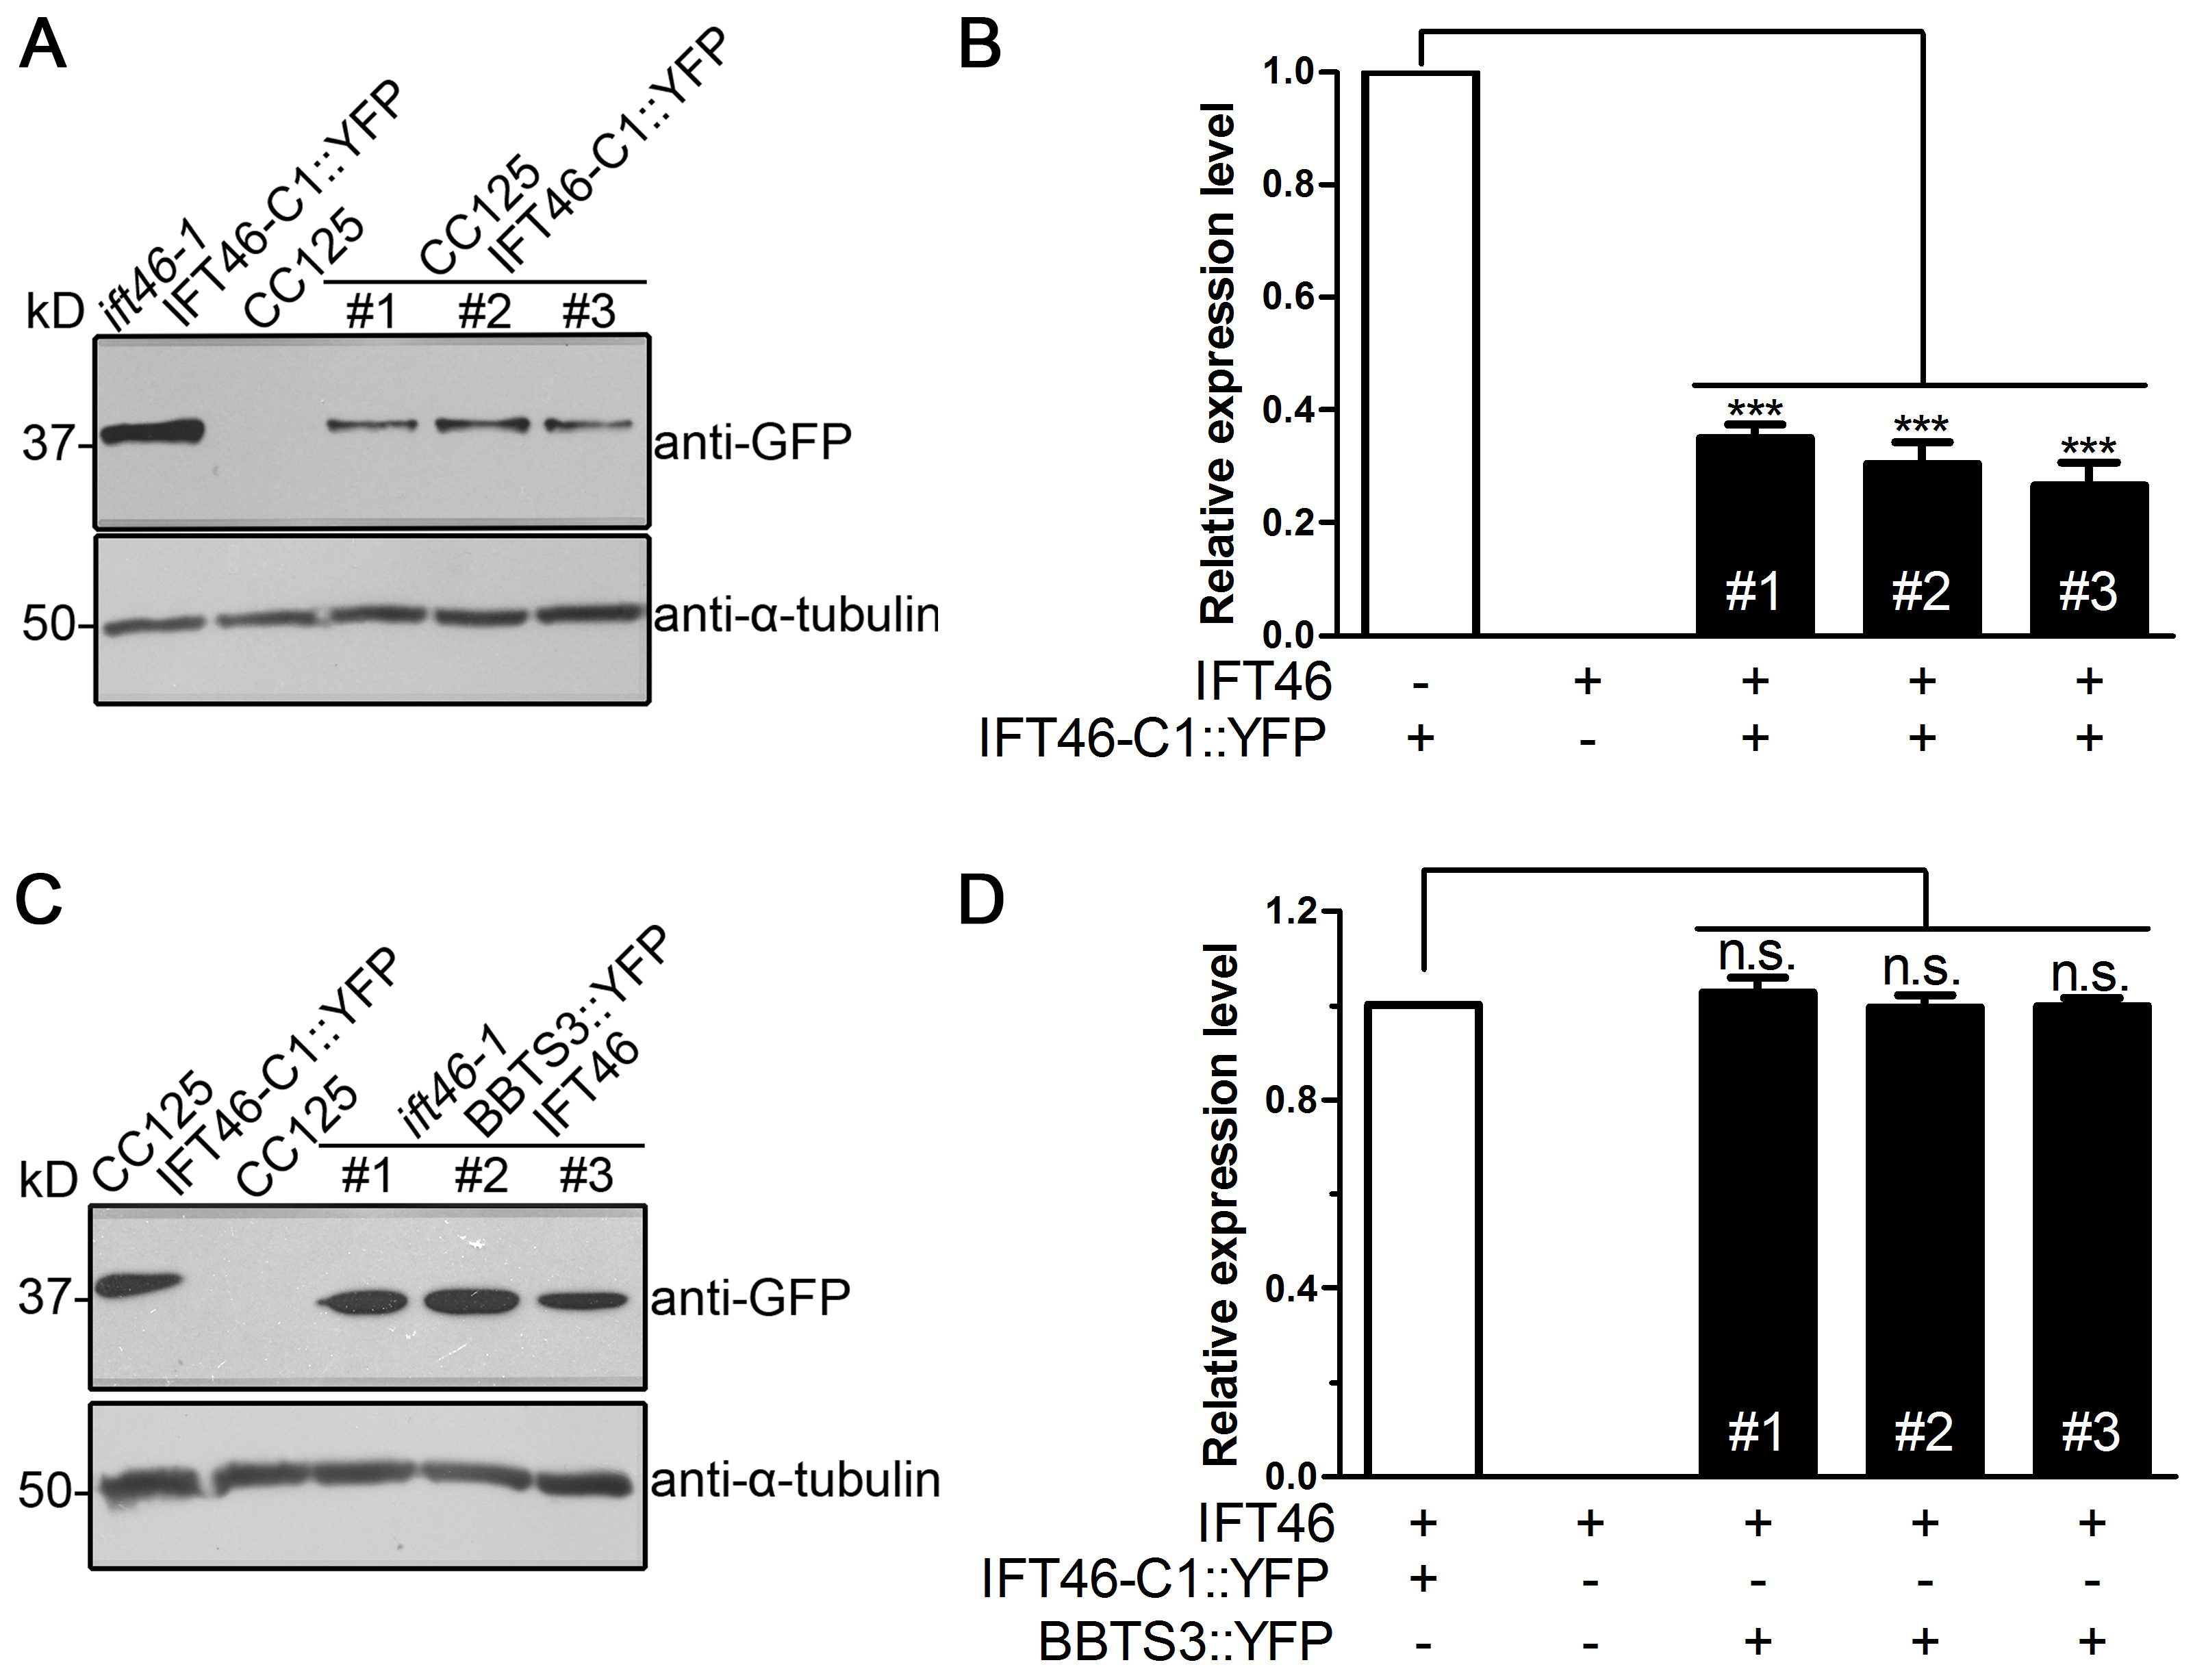
\includegraphics[width=\textwidth]{fig4-9.jpg}
%生成中英双语标题
{\setstretch{1.667}
\bicaption[fig:4.9]{图}{IFT46-C1\ 和\ BBTS3\ 在全长\ IFT46\ 存在的条件下表达水平的变化。(A)\textit{ift46-1} \textit{IFT46-C1::YFP}、CC-125\ 和\ CC-125 \textit{IFT46-C1::YFP}\ 全细胞裂解液免疫印迹分析。(B)IFT46-C1::YFP\ 在\ CC-125\ 和\ \textit{ift46-1}\ 中的相对表达水平。(C)CC-125 \textit{IFT46-C1::YFP}、CC-125\ 和\ \textit{ift46-1} \textit{BBTS3::YFP IFT46}\ 全细胞裂解液免疫印迹分析。(D)BBTS3::YFP\ 在\ \textit{ift46-1} \textit{BBTS3::YFP IFT46}\ 中与\ IFT46-C1::YFP\ 在\ CC-125\ 中表达水平的比较。}{Figure}{The expression level of IFT46-C1 and BBTS3 in the presence of full-length IFT46. (A)	Western blots of whole-cell lysates (3 $\upmu$g protein per lane) of \textit{ift46-1} \textit{IFT46-C1::YFP}, CC-125, and CC-125 \textit{IFT46-C1::YFP} probed with the indicated antibodies. (B) Relative expression level of IFT46-C1::YFP in CC-125 in three transformants compared to the expression level of IFT46-C1::YFP in \textit{ift46-1}. (C) Western blots of whole-cell lysates (3 $\upmu$g protein per lane) of CC-125 \textit{IFT46-C1::YFP}, CC-125, and \textit{ift46-1} \textit{BBTS3::YFP IFT46} probed with the indicated antibodies. (D) Relative expression level of BBTS3::YFP in \textit{ift46-1} \textit{BBTS3::YFP IFT46} in three transformants compared to the expression level of IFT46-C1::YFP in CC-125.}
\par}
%结束图片浮动体环境
\end{figure}

%开始图片浮动体环境,其中!表示取消严谨限制,h表示在此处插入,t表示在本页或下一页顶部插入
\begin{figure}[htbp]
%居中对齐
\centering
%设置图片搜索路径,每个路径用{}括起来
\graphicspath{{figures/}}
%插入图片并设置图片宽度为文本宽度减10mm
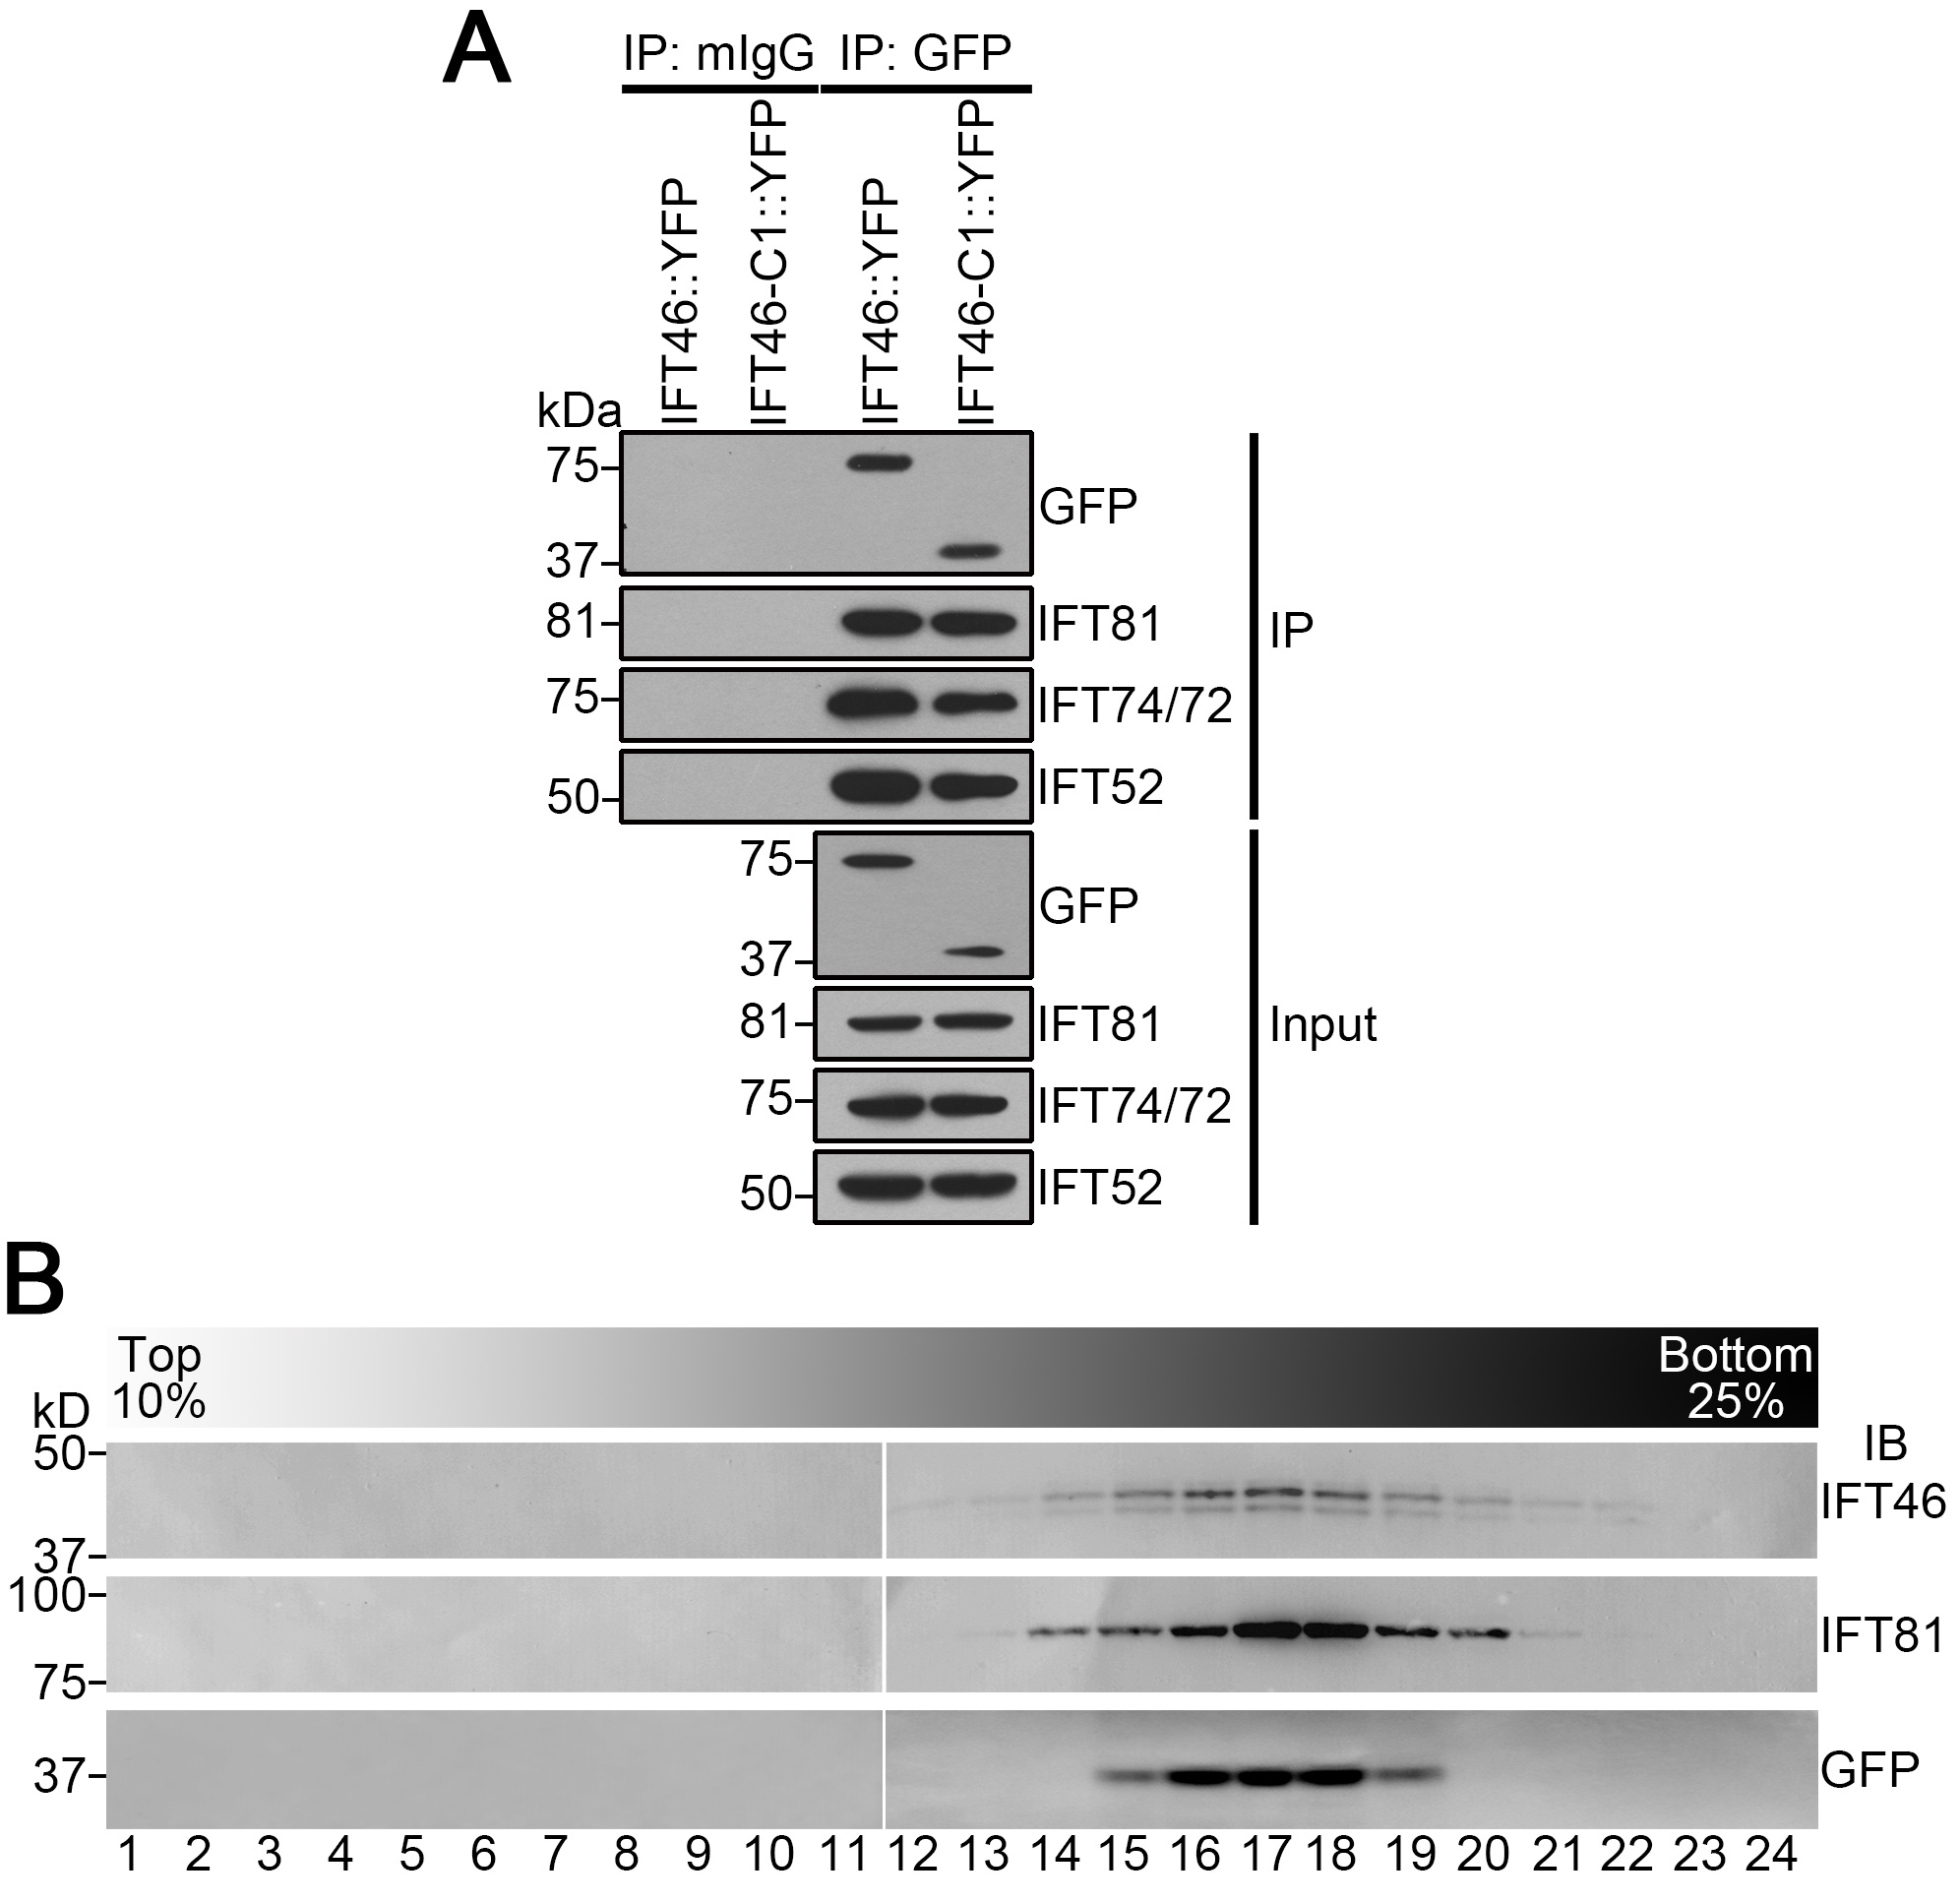
\includegraphics[width=\textwidth-30mm]{fig4-11.jpg}
%生成中英双语标题
{\setstretch{1.667}
\bicaption[fig:4.11]{图}{IFT46-C1\ 组装在IFT复合物中。(A)以\ \textit{ift46-1} \textit{IFT46::YFP}\ 和\ CC-125\ \textit{IFT46-C1::YFP}\ 和鞭毛膜/基质为材料,使用抗\ GFP\ 的抗体免疫沉淀带\ YFP\ 标签的\ IFT46-C1。 使用抗\ IFT81、IFT74/72\ 和\ IFT52\ 的抗体进行检测。mIgG\ 代表鼠\ IgG。 (B)使用蔗糖密度梯度离心对\ CC-125 \textit{IFT46-C1::YFP}\ 的鞭毛膜/基质部分进行分析。图中抗\ IFT46\ 的抗体检测到两条带是磷酸化造成的。IB\ 代表免疫印迹。图片下方的数字为组分编号。}{Figure}{IFT46-C1 is assembled into IFT machinery. (A) Anti-GFP antibody was used to immunopreciptate YFP-tagged IFT46-C1 from the flagellar membrane-plus-matrix of \textit{ift46-1} \textit{IFT46::YFP} and CC-125 \textit{IFT46-C1::YFP}. Immunoblots of the precipitate were probed with antibodies against IFT81, IFT74/72 and IFT52. mIgG: mouse IgG; IP: immunoprecipitation. (B)	Flagellar membrane-plus-matrix of CC-125 \textit{IFT46-C1::YFP} was separated by sucrose density gradient centrifugation and analyzed by immunoblots probed with antibodies as indicated. IFT46 migrates as doublet bands due to phosphorylation. IB: immunoblot. Numbers at the bottom indicate fractions.}
\par}
%结束图片浮动体环境
\end{figure}

\section{讨论}
本章我们通过在\ \textit{IFT46}\ 的缺失突变体\ \textit{ift46-1}\ 和野生型\ CC-125\ 细胞中表达\ IFT46\ 的截短片段成功鉴定到\ IFT46\ 的基体和纤毛定位序列。IFT46-C1\ 可被认为是\ IFT46\ 的基体和纤毛定位序列,因为它满足下列标准。一,IFT46-C1\ 是\ IFT46\ 基体定位所必须的。当\ IFT46-C1\ 被删除的时候,IFT46$\Delta$C1\ 无法定位在基体和鞭毛(图\ \ref{fig:4.6})。二,IFT46-C1\ 能够将与鞭毛无关的蛋白\ YFP\ 靶向至基体和纤毛(图\ \ref{fig:4.6})。以上事实表明,IFT46-C1\ 是\ IFT46\ 基体和纤毛定位的充分必要条件。然而,与其他定位序列相比(如\ GPCRs\ 的第三个胞内、Ax(S/A)xQ、RVxP、核定位信号以及\ SUMOylation\ 等),IFT46-C1\ 的长度明显偏大\
\citep{Malicki2014,Bhogaraju2013,McIntyre2015,Dishinger2010,Berbari2008,Hurd2011,Santos2014}。 这表明参与\ IFT46\ 基体定位的蛋白运输系统不是这些已知途径。考虑到\ IFT46-C1\ 和\ BBTS3\ 能够进入纤毛且沿轴丝做双向运动,IFT46-C1\ 或\ BBTS3\ 可能通过与其他IFT亚基形成复合物完成基体和纤毛定位。

我们同时发现\ IFT46-C1\ 和\ BBTS3\ 均为\ IFT46\ 的基体和纤毛定位序列(
图\ \ref{fig:4.6}、\ref{fig:4.8})。在全长\ IFT46\ 存在的条件下,IFT46-C1\ 和\ BBTS3\ 的表达量均下降至原来的\ 30\%(图\ \ref{fig:4.9})。然而,在全长\ IFT46\ 存在的情况下,BBTS3\ 在传代过程中更容易丢失或沉默。考虑到\ BBTS3\ 仅比\ IFT46-C1\ 少一段甘氨酸尾巴(图\ \ref{fig:4.4}),我们推测\ IFT46\ 的甘氨酸尾巴可能有助于维持其稳定。IFT46\ 的甘氨酸尾巴为动态无序区,其N端也为动态无序结构
(图\ \ref{fig:4.3})。研究表明\ IFT46\ 的\ N\ 端可增强\ IFT46\ 与\ ODA16\ 之间的相互作
用\ \citep{Ahmed2008,Ahmed2005,Taschner2011,Hou2007}。因此,IFT46\ 的甘氨酸尾巴可能通过增强\ IFT46\ 与其他蛋白如\ IFT52\ 之间的相互作用来提高其稳定性\ \citep{Lv2017}。

我们表达的\ IFT46\ 截短片段均无法拯救或部分拯救\ \textit{ift46-1}\ 的鞭毛缺失表型。然而,
\textit{IFT46}\ 的部分抑制突变体\ \textit{Sup$_{ift46}$1}\ 在缺氧压力条件下可形成长鞭毛\ \citep{Hou2007}。在\ \textit{Sup$_{ift46}$1}\ 中,MRC1\footnote{miniature retrotransposon of \textit{Chlamydomonas}}\ 转座子的插入使得\ IFT46\ 的\ C\ 端\ 240\ 个氨基酸(105-344)得以表达\ \citep{Hou2007}。类似的,在\ \textit{ift46-1}\ 中表达\ IFT46\ 的\ C\ 端(106-344)获得的藻株\
\textit{ift46-1 IFT46$\Delta$105}\ 在压力条件下也能够长出长鞭毛\ (Hou and Witman, 2017; 未发表)。这种不一致情况的出现可能是由藻株的培养条件不同导致的。\textit{Sup$_{ift46}$1}\ 和\ \textit{ift46-1 IFT46$\Delta$105}\ 均需要在曝气条件下培养至对数生长期然后静置培养才能缓慢长出鞭毛\ (Hou and Witman, 2017; 未发表)。即使如此,
\textit{Sup$_{ift46}$1}\ 和\ \textit{ift46-1 IFT46$\Delta$105}\ 的鞭毛率也远低于野生型细胞\ (Hou and Witman, 2017; 未发表)。压力条件能够促使鞭毛缺失突变体重新长出鞭毛的现象并非首次被观察到,其确切原因暂时未知\ (Hou and Witman, 2017; 未发表)。

此外,我们在实验过程中发现\ IFT46\ 存在磷酸化修饰。根据\ Joel Rosenbaum\ 实验室未发表的结果,\ IFT46\ 的磷酸化对纤毛形成和纤毛功能是非必须的。将衣藻\ IFT46\ 的磷酸化位点突变为无法磷酸化的氨基酸残基对纤毛相关表型无明显影响。IFT46\ 的磷酸化可能在其参与非纤毛功能的过程中发挥作用。根据这些结果,我们在研究中并未关注\ IFT46\ 的磷酸化。衣藻细胞中磷酸化\ IFT46\ 的含量不稳定且偏低,一般需要通过蔗糖密度梯度聚丙烯酰氨凝胶电泳才能分辨。这可能是我们有时能检测到磷酸化条带的原因之一。此外,我们无法排除\ IFT46\ 存在其他翻译后修饰的可能。

\section{小结}
通过表达截短片段的方式我们发现\ IFT46-C1\ 和\ BBTS3\ 是\ IFT46\ 的基体定位序列,同时它们也是\ IFT46\ 的纤毛定位序列。此外我们还发现\ IFT46-C1\ 可通过与\ IFT-B\ 复合物中的其他亚基相互作用形成复合物。这暗示我们\ IFT46\ 的基体和纤毛定位可能与其他\ IFT\ 亚基有关。